\documentclass[12pt,a4paper]{article}

\usepackage[utf8]{inputenc}
\usepackage[T1]{fontenc}
\usepackage[ngerman]{babel}
\usepackage{lmodern}
\usepackage[a4paper,left=3cm,right=2cm,top=2.5cm,bottom=2cm]{geometry}
\usepackage{setspace}
\usepackage{graphicx}
\usepackage{booktabs}
\usepackage{array}
\usepackage{tabularx}
\usepackage{longtable}
\usepackage{ragged2e}
\usepackage{caption}
\usepackage{eurosym}
\usepackage[hidelinks]{hyperref}

% text-wrapping X column, left-aligned
\newcolumntype{Y}{>{\RaggedRight\arraybackslash}X}

\setstretch{1.5}
\captionsetup{font=small,labelfont=bf}
\setlength{\parindent}{0pt}
\setlength{\parskip}{0.6em}

% ---- Titelblatt-Platzhalter: hier einmal ausfüllen ----
\newcommand{\standort}{[Standort]}
\newcommand{\studiengang}{[Studiengang]}
\newcommand{\matrikelnummer}{[Matrikelnummer]}

\begin{document}

\begin{titlepage}
\centering
{\large FOM Hochschule für Oekonomie \& Management\par}
{\large Hochschulzentrum \standort\par}
\vspace{2.5cm}
{\large Projektarbeit\par}
{\large im Modul \glqq ERP-Systeme\grqq{}\par}
{\large im Studiengang \studiengang\par}
\vspace{1.5cm}
{\large über das Thema\par}
\vspace{0.8cm}
{\Large\bfseries Analyse von Prozessineffizienzen durch Process Mining in ERP-Systemen:\\[0.3cm]
Eine Untersuchung der Datenstrukturen und Algorithmen am Beispiel des Order-to-Cash-Prozesses\par}
\vspace{1.5cm}
{\large Betreuer: Dipl.-Ing. Sandro Coletta\par}
\vfill
{\large von\par}
{\large\bfseries Tom Potthoff\par}
{\large Matrikelnummer: \matrikelnummer\par}
\vspace{0.8cm}
{\large Abgabedatum: 16.07.2026\par}
\end{titlepage}


\clearpage
\pagenumbering{Roman}
\tableofcontents
\clearpage
\listoffigures
\listoftables
\clearpage

\phantomsection\addcontentsline{toc}{section}{Abkürzungsverzeichnis}
\section*{Abkürzungsverzeichnis}
{\small
\begin{longtable}{@{}>{\bfseries}l l@{}}
\toprule
AT & Arbeitstag(e) \\
BPI & Business Process Intelligence (Challenge) \\
CO & Controlling (SAP-Modul) \\
CSV & Comma-Separated Values (Textdatenformat) \\
DFG & Directly-Follows-Graph (Abfolgegraph) \\
DSO & Days Sales Outstanding (Forderungslaufzeit) \\
ECC & ERP Central Component (SAP-Vorgängersystem) \\
EDI & Electronic Data Interchange \\
ERP & Enterprise Resource Planning \\
FI & Financial Accounting (SAP-Modul) \\
FSCM & Financial Supply Chain Management \\
GiGo & Garbage in, Garbage out \\
IDoc & Intermediate Document (SAP-Nachrichtenformat) \\
KPI & Key Performance Indicator \\
MM & Materials Management (SAP-Modul) \\
O2C & Order-to-Cash \\
PP & Production Planning (SAP-Modul) \\
SD & Sales and Distribution (SAP-Modul) \\
VZÄ & Vollzeitäquivalent \\
WA & Warenausgang \\
XES & eXtensible Event Stream (IEEE-Standard 1849-2016) \\
\bottomrule
\end{longtable}}


\clearpage
\pagenumbering{arabic}

% Tabellen-/Abbildungszaehler nach dem Frontmatter zuruecksetzen
% (die longtable im Abkuerzungsverzeichnis erhoeht sonst den Tabellenzaehler)
\setcounter{table}{0}
\setcounter{figure}{0}

\chapter{Einleitung}\label{ch:einleitung}


\section{Problemstellung und Motivation}\label{sec:problemstellung}

\gls{erp}-Systeme sind das zentrale Anwendungssystem für den betrieblichen Alltag. Sie umfassen nach Gronau die Verwaltung aller zur Durchführung von Geschäftsprozessen notwendigen Informationen über die Ressourcen Material, Personal, Kapazitäten, Finanzen und Informationen und setzen dafür eine gemeinsame Datenhaltung voraus\footcite[Vgl.][S.~4]{gronau2014erp}. Auf der operativen Ebene führen sie die täglichen Routinetransaktionen des Geschäftsbetriebs aus und zeichnen diese auf\footcite[Vgl.][S.~125 ff.]{vanderaalst2016processmining}. Jeder Beleg, jede Buchung und jede Änderung hinterlässt dabei in der zentralen Datenbank eine digitale Spur mit Zeitstempel. Process Mining macht diese Spuren nutzbar und analysiert Geschäftsprozesse nicht so, wie sie dokumentiert sind, sondern so, wie sie tatsächlich ablaufen\footcites(Vgl.)()[S.~169 f.]{vanderaalst2012manifesto}[S.~13]{adolfsson2026o2c}.

Untersuchungsgegenstand ist der \gls{o2c} im Vertriebsmodul \gls{sd} von \gls{sap} \gls{s/4hana}. Er umfasst die Prozesskette von der Auftragsaufnahme über Verfügbarkeitsprüfung, Kommissionierung und Versand bis zur Fakturierung und zum Zahlungseingang\footcite[Vgl.][]{SAP_Verkaufsanalyse} und verläuft als erlöswirksamer End-to-End-Prozess abteilungsübergreifend durch Vertrieb, Lager und Finanzbuchhaltung\footcite[Vgl.][S.~63 ff.]{scheibler2021vertrieb}. Sein hohes Belegvolumen, die unmittelbare Wirkung auf Kundenzufriedenheit und Liquidität sowie die vollständige Abbildung im \gls{erp}-System eignen ihn gut für eine Process-Mining-Analyse. Zugleich gilt der \gls{o2c}-Prozess als einer der am besten standardisierten und zugleich am häufigsten durch gewachsene Sonderregelungen überformten Prozesse, sodass sich an ihm besonders deutlich zeigt, wie weit dokumentierter Soll-Ablauf und tatsächliche Ausführung auseinanderfallen können.

In der beruflichen Praxis der Auftragsabwicklung zeigen sich regelmäßig die typischen Symptome ineffizienter \gls{o2c}-Prozesse: Aufträge, die in Kredit- oder Liefersperren hängen bleiben, Klärungsschleifen zwischen Vertrieb und Versand nach Auftragsänderungen sowie Rechnungen, die das Haus erst Tage nach dem Warenausgang verlassen. Auch die Fachliteratur zu \gls{sap} \gls{sd} benennt manuelle Dateneingabe, fragmentierte Informationssysteme und verzögerte Auftragsabwicklung als wiederkehrende Schwachstellen\footcite[Vgl.][S.~109 f.]{nadukuru2024o2c}. Dieselbe Literatur identifiziert Automatisierung, Datenintegration und fortgeschrittene Analytik als die zentralen Hebel, um diese Schwächen zu beheben, und ordnet damit die datengetriebene Prozessanalyse in eine breitere Optimierungsagenda ein\footcite[Vgl.][S.~110 ff.]{nadukuru2024o2c}. Versuche, solche Ursachen in Prozessworkshops zu erheben, bleiben erfahrungsgemäß unbefriedigend, weil die Beteiligten denselben Prozess unterschiedlich beschreiben und die Prozessdokumentation häufig unvollständig ist\footcite[Vgl.][S.~50 und 62]{adolfsson2026o2c}. Process Mining stützt die Analyse stattdessen auf Daten: Die Ergebnisse sind faktenbasiert und intersubjektiv nachvollziehbar, weil sie unmittelbar aus den Aufzeichnungen des Systems gewonnen werden\footcite[Vgl.][S.~169 ff.]{vanderaalst2012manifesto}.

Bewusst wird kein reales Unternehmen untersucht, sondern ein offen dokumentierter Datensatz. Die Datenstrukturen und Algorithmen des Process Mining lassen sich an einem reproduzierbaren Event-Log präziser untersuchen als an vertraulichen Unternehmensdaten, deren Freigabe zudem datenschutzrechtliche und arbeitsrechtliche Fragen aufwerfen würde. Die Datengrundlage wird in Kapitel~\ref{sec:datengrundlage} eingeordnet und begründet.

\section{Zielsetzung und Forschungsfragen}\label{sec:zielsetzung}

Ziel der Arbeit ist es, zu untersuchen, wie Prozessineffizienzen in \gls{erp}-Systemen mittels Process Mining identifiziert werden können. Dazu werden drei Leitfragen verfolgt:
\begin{enumerate}
    \item Welche Datenstrukturen eines \gls{sap}-Systems liefern die Rohdaten für ein Process-Mining-taugliches Ereignisprotokoll (Event-Log), und wie wird dieses daraus gewonnen?
    \item Welche Algorithmen stehen für die Prozessentdeckung und den Soll-Ist-Abgleich zur Verfügung, und wie schlagen sie sich im praktischen Vergleich auf einem realistischen \gls{o2c}-Log?
    \item Welche Prozessineffizienzen lassen sich in dem analysierten Log quantifizieren, und mit welchen Anpassungen im \gls{sap}-System ließen sie sich beheben?
\end{enumerate}
Da der verwendete Log synthetisch erzeugt wird, die injizierten Störungsmuster also vorab bekannt sind, dient die Analyse zugleich als Methodenvalidierung. Ein taugliches Analyseverfahren muss die bekannte Grundwahrheit aus den Daten zurückgewinnen. Methodisch folgt die Arbeit damit dem Grundgedanken der gestaltungsorientierten Wirtschaftsinformatik, in der ein Artefakt, hier die Extraktions- und Analysemethode, konstruiert und anschließend an einem nachprüfbaren Maßstab evaluiert wird. Sie liefert damit nicht nur eine Fallstudie, sondern einen überprüfbaren Nachweis, dass sich aus den Standard-Datenstrukturen eines \gls{sap}-Systems belastbare Prozessdiagnosen gewinnen lassen. Der Anspruch der Arbeit ist damit ausdrücklich ein methodischer: Nicht die Behebung eines konkreten Einzelfalls steht im Vordergrund, sondern der nachvollziehbare Nachweis eines übertragbaren, beratungsorientierten Vorgehens.

\section{Vorgehensweise und Aufbau der Arbeit}\label{sec:vorgehensweise}

Die Arbeit folgt der funktionalen Gliederung in Einleitung, Grundlagen, Umsetzung und Schluss. Kapitel~\ref{ch:grundlagen} legt die Grundlagen: den \gls{o2c}-Prozess mit seinen typischen Schwachstellen, seinen Aufbau im Modul \gls{sd} mit Strukturen, Stamm- und Bewegungsdaten sowie die Konzepte und Algorithmen des Process Mining. Kapitel~\ref{ch:umsetzung} bildet die Umsetzung und damit den Kern der Arbeit: Aus den \gls{sap}-Datenstrukturen wird ein Event-Log konstruiert, auf dem Discovery- und Conformance-Verfahren ausgeführt und die Ineffizienzen quantifiziert werden. Kapitel~\ref{ch:empfehlungen} leitet daraus beratungsorientierte Handlungsempfehlungen einschließlich einer Implementierungsstrategie ab. Kapitel~\ref{ch:fazit} fasst die Ergebnisse entlang der drei Forschungsfragen zusammen und gibt einen Ausblick.

\chapter{Beschreibung des aktuellen Prozesses}\label{ch:prozessbeschreibung}


\section{\gls{erp}-Systeme als Datenquelle des Process Mining}\label{sec:erp-grundlagen}

Um den Untersuchungsgegenstand einzuordnen, sind einige Grundbegriffe zu klären. Ein Anwendungssystem besteht aus \gls{it}-Infrastruktur, Anwendungssoftware und Daten \parencite[Folie~16]{coletta2026_0303}. Anwendungssysteme lassen sich nach Organisationsebenen unterscheiden: Auf der operativen Ebene führen sie die täglichen Routinetransaktionen aus und zeichnen sie auf, darüber liegen Management-Informationssysteme für Standardberichte sowie Entscheidungs- und Führungsunterstützungssysteme für schwächer strukturierte Entscheidungen \parencite[Folie~33--39]{coletta2026_0303}. \gls{erp}-Systeme sind der prototypische Vertreter der operativen Ebene, und weil dort jede Transaktion protokolliert wird, entsteht dort auch das Rohmaterial für spätere Analysen.

Der Begriff \gls{erp} ist historisch gewachsen. Aus einfachen Systemen der Materialbedarfsplanung (MRP) entwickelte sich über die Zwischenstufe MRP\,II die integrierte Unternehmensplanung, die Vertrieb, Finanzwesen, Warenwirtschaft und Controlling zusammenführte \parencite[Folie~43]{coletta2026_0303}. Entscheidend für die vorliegende Arbeit ist die Integration: Betriebliche Anwendungssysteme lassen sich horizontal, entlang der Prozesskette über Funktionsbereiche hinweg, und vertikal, über die Führungsebenen, integrieren, und diese Integration setzt eine gemeinsame Datenhaltung voraus \parencites[S.~4]{gronau2014erp}[Folie~44 und 48]{coletta2026_0303}. Ein wesentlicher Nutzen von \gls{erp}-Systemen besteht denn auch darin, dass sich Informationssilos öffnen und vormals getrennte Teilprozesse miteinander verzahnt werden \parencite[Folie~74]{coletta2026_1003}.

Für Process Mining ist diese Eigenschaft fundamental. Weil ein Kundenauftrag nicht in mehreren getrennten Abteilungssystemen, sondern in einer integrierten Datenbank abgewickelt wird, hinterlässt er dort seine vollständige, lückenlose Spur, vom ersten Beleg bis zum Zahlungsausgleich. Ohne diese Integration wäre die Rekonstruktion eines durchgängigen Prozessablaufs praktisch unmöglich, mit ihr wird sie zur reinen Datenextraktionsaufgabe. Das \gls{erp}-System ist damit nicht nur das System, das den Prozess ausführt, sondern zugleich das System, das ihn dokumentiert. Ergänzend ist \gls{erp}-Software Standardsoftware mit vordefinierten, an Best Practices orientierten Geschäftsprozessen, die per Customizing an das Unternehmen angepasst werden \parencite[Folie~41]{coletta2026_0303}. Zwei Unternehmen mit derselben Software können daher völlig unterschiedliche Ist-Prozesse aufweisen, nicht weil die Software verschieden wäre, sondern weil sie unterschiedlich konfiguriert und genutzt wird. Genau diese Lücke zwischen vorgesehenem Standard und tatsächlicher Nutzung ist der Gegenstand der Fit/Gap-Analyse in Kapitel~\ref{ch:fitgap}, für die Process Mining die empirische Grundlage liefert.

Diese integrierte Datenhaltung unterscheidet operative \gls{erp}-Systeme grundlegend von analytischen Systemen wie einem Data Warehouse, das Daten für Auswertungszwecke aus den operativen Beständen extrahiert und aufbereitet. Process Mining nimmt eine Zwischenstellung ein: Es wertet operative Belegdaten aus, benötigt dafür aber, ähnlich einem Data-Warehouse-Ladeprozess, einen vorgeschalteten Extraktions- und Aufbereitungsschritt \parencite[Folie~400 f.]{coletta2026_2306}. Genau dieser Schritt, die Rekonstruktion eines Event-Logs aus den Belegtabellen, steht im Zentrum von Kapitel~\ref{sec:datenstrukturen}.


\section{Der \gls{o2c}-Prozess und seine typischen Schwachstellen}\label{sec:o2c-schwachstellen}

Der untersuchte Prozess folgt dem klassischen Ablauf der Auftragsabwicklung. Ein eingehender Kundenauftrag wird im Vertriebsinnendienst erfasst, durchläuft eine Kreditprüfung, wird zur Logistik freigegeben, dort kommissioniert und mit Warenausgang ausgeliefert, anschließend fakturiert und durch den Zahlungseingang abgeschlossen \parencite[Folie~62 f.]{coletta2026_0303}. Abbildung~\ref{fig:o2c-prozess-stoerungsmuster} zeigt den Prozess mit sechs in der betrieblichen Praxis immer wieder beobachteten Störungsmustern: nachträgliche Auftragsänderungen mit Klärungsschleifen (K1) \parencites[S.~55]{adolfsson2026o2c}[S.~109 f.]{nadukuru2024o2c}, manuelle Kreditprüfungen mit Liegezeiten (K2) \parencites[S.~63 ff.]{scheibler2021vertrieb}[S.~3 ff.]{reinkemeyer2020processmining}, Liefersperren infolge lückenhafter Kundenstammdaten (K3) \parencites[S.~55 f.]{adolfsson2026o2c}[S.~63 ff.]{scheibler2021vertrieb}, Fakturierung nur im wöchentlichen Sammellauf (K4) \parencites[S.~109 f.]{nadukuru2024o2c}[S.~3 ff.]{reinkemeyer2020processmining}, Fakturasperren durch manuell im Auftrag geänderte Preise (K5) \parencites[S.~55 f.]{adolfsson2026o2c}[S.~63 ff.]{scheibler2021vertrieb} sowie Reklamationen mit Gutschrift und Nachlieferung nach Falschlieferungen (K6) \parencites[S.~21 ff.]{peters2019processmining}[S.~109 f.]{nadukuru2024o2c}. Diese sechs Muster bilden die Grundwahrheit der Untersuchung. Sie werden kontrolliert injiziert (Kapitel~\ref{sec:datengrundlage}) und müssen in Kapitel~\ref{ch:fitgap} wiedergefunden und quantifiziert werden.

\begin{figure}[!htb]
\centering
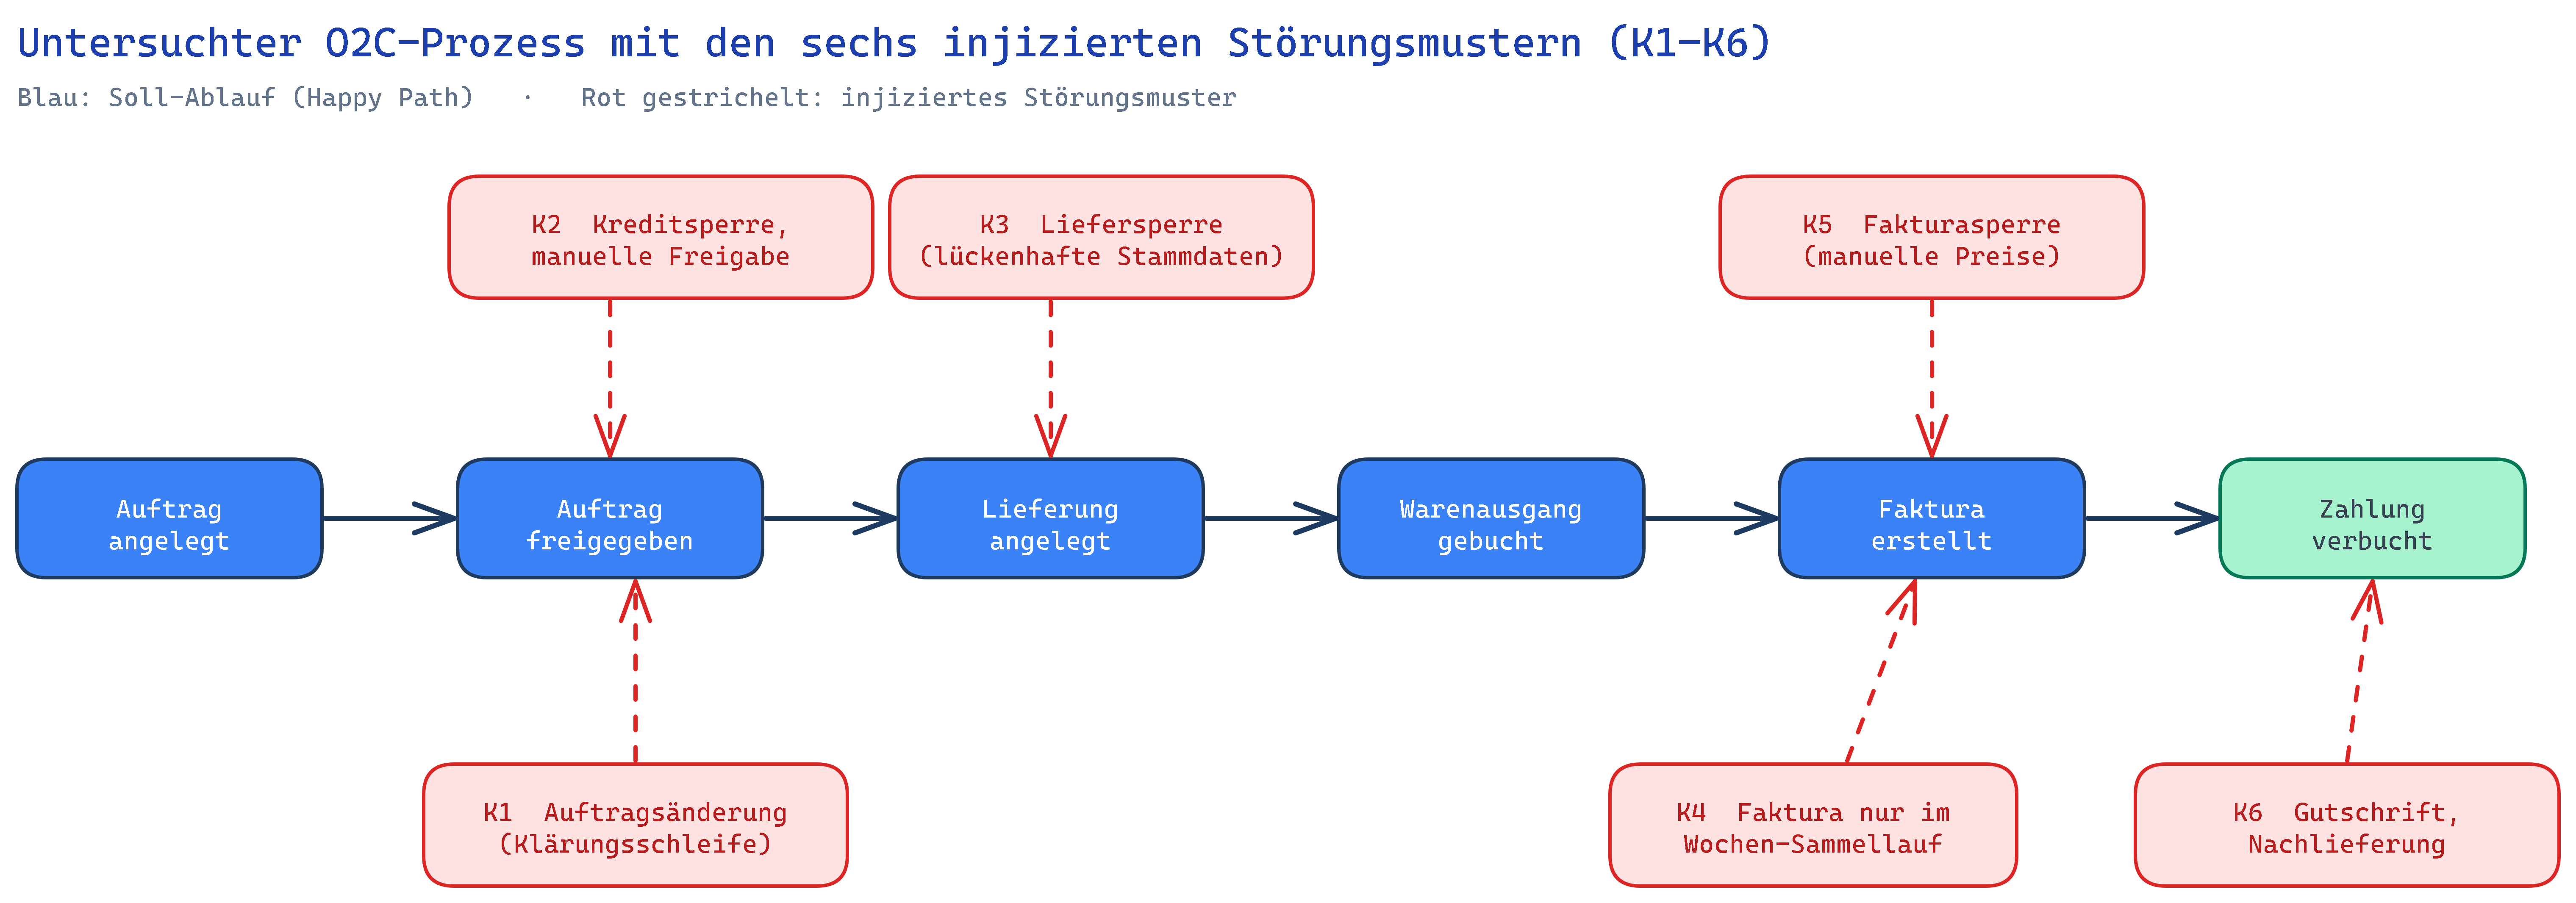
\includegraphics[width=\textwidth,height=0.36\textheight,keepaspectratio]{figures/image1.png}
\caption{Untersuchter O2C-Prozess mit den sechs injizierten Störungsmustern K1--K6 (Quelle: eigene Darstellung)}\label{fig:o2c-prozess-stoerungsmuster}
\end{figure}

Jedes dieser Muster ist für sich genommen harmlos und oft sogar gut gemeint, denn eine Kreditprüfung schützt vor Forderungsausfällen und eine Liefersperre vor Fehllieferungen. Problematisch werden sie erst durch ihre Häufigkeit und durch die Liegezeiten, die sie erzeugen. Genau diese quantitative Dimension, wie oft ein Muster auftritt, wie viel Zeit es kostet und welche Fälle betroffen sind, lässt sich in Workshops nicht zuverlässig erheben, wohl aber aus den Zeitstempeln des \gls{erp}-Systems messen. Der Beitrag des Process Mining liegt somit weniger im Entdecken der Existenz solcher Muster als in ihrer objektiven Vermessung und Priorisierung.

Ein Beispiel verdeutlicht das Zusammenspiel der Muster. Ein Bestandskunde bestellt freitags dringend benötigte Ware. Der Auftrag wird noch am selben Tag erfasst, läuft jedoch in die Kreditsperre (K2), weil ein statisches Limit rechnerisch überschritten ist. Die manuelle Freigabe erfolgt erst am Montag, die Lieferung verlässt das Werk am Mittwoch, und die Rechnung entsteht erst im Sammellauf der Folgewoche (K4). Zwischen Bestellung und Faktura vergehen so über zehn Kalendertage, ohne dass ein Beteiligter einen Fehler gemacht hätte. Die Verzögerung ist vollständig prozess- und konfigurationsbedingt und damit genau die Art von Ineffizienz, die eine datenbasierte Analyse sichtbar und messbar macht.

Kennzeichnend für den \gls{o2c}-Prozess ist zudem seine abteilungsübergreifende Natur. Der Vertrieb verantwortet Auftragserfassung und Freigabe, das Lager Kommissionierung und Warenausgang, die Finanzbuchhaltung Faktura, Zahlungseingang und Mahnwesen. Jeder Übergang zwischen diesen Bereichen ist eine potenzielle Bruchstelle, an der Wartezeiten, Rückfragen oder Medienbrüche entstehen. Gerade weil kein einzelner Bereich den Gesamtprozess überblickt, entzieht sich dessen tatsächlicher Verlauf der Wahrnehmung der Beteiligten, und gerade deshalb ist eine systemübergreifende, datenbasierte Rekonstruktion so aufschlussreich.

\section{Datengrundlage -- öffentliche und synthetische Event-Logs}\label{sec:datengrundlage}

Öffentliche Real-Logs wie der \gls{bpi}-Challenge-2019-Log erlauben Process-Mining-Untersuchungen ohne Zugriff auf vertrauliche Unternehmensdaten. Dieser dokumentiert den Bestellabwicklungsprozess (Purchase-to-Pay) eines multinationalen Konzerns mit rund 1,6 Millionen Ereignissen zu etwa 250.000 Bestellpositionen \parencite{vandongen2019bpi}. Für die vorliegende Fragestellung ist er nur eingeschränkt geeignet, weil er den Einkaufs- und nicht den Vertriebsprozess abbildet und die tatsächlichen Prozessschwächen des anonymen Konzerns unbekannt sind, eine Validierung gegen eine Grundwahrheit also unmöglich ist. Die Analyse realer Firmendaten, wie sie die \gls{o2c}-Fallstudie von Adolfsson/Saleh am Lebensmittelkonzern Paulig durchführt, erfordert wiederum genau den vertraulichen Zugang, den diese Arbeit meidet, und besitzt ebenfalls keine bekannte Grundwahrheit \parencite[S.~4 ff.\ und 28]{adolfsson2026o2c}.

Die Arbeit nutzt daher einen synthetischen \gls{sap}-\gls{o2c}-Event-Log, der mit einem Python-Simulationsskript erzeugt und mit der Open-Source-Bibliothek \gls{pm4py} verarbeitet wird \parencite{berti2019pm4py}. Simuliert werden 12.000 Kundenaufträge eines Geschäftsjahres (01.07.2025 bis 30.06.2026) entlang des \gls{sap}-Belegflusses aus Kapitel~\ref{ch:sap-prozessanalyse}, wobei die sechs Störungsmuster aus Abbildung~\ref{fig:o2c-prozess-stoerungsmuster} mit festen Wahrscheinlichkeiten und Verzögerungsverteilungen injiziert werden (Parameter in Anhang A2). Der resultierende Log umfasst 84.121 Ereignisse zu elf Aktivitätstypen und wird als \gls{csv}-Tabelle und im \gls{xes}-Format exportiert. Durch den festen Zufalls-Seed 42 ist das Vorgehen vollständig reproduzierbar, es erfordert keine Firmenfreigabe und wirft keine Datenschutzfragen auf, weil alle Benutzerkennungen synthetisch sind. An die Stelle des in der Aufgabenstellung skizzierten fiktiven Unternehmens tritt damit bewusst ein offengelegter, reproduzierbarer Datensatz, die vorgegebene Kapitelstruktur bleibt davon unberührt. Der Preis ist, dass der Log modelliertes und kein real gewachsenes Verhalten zeigt, worauf in Kapitel~\ref{ch:zusammenfassung} zurückzukommen ist.

Methodisch wird jedes Störungsmuster als bedingte Verzweigung in den Generierungsprozess eingebaut. Mit der jeweiligen Wahrscheinlichkeit aus Anhang A2 wird pro Fall entschieden, ob etwa eine Kreditsperre gesetzt wird, und die zugehörige Liegezeit wird aus einer Lognormalverteilung über Arbeitstage gezogen, sodass sich realistische, rechtsschiefe Wartezeiten mit vielen kurzen und wenigen sehr langen Verzögerungen ergeben. Weil die Wahrscheinlichkeiten und Verteilungen bekannt sind, ist die erwartete Häufigkeit jedes Musters vorab bestimmbar, und die spätere Analyse muss diese Erwartung reproduzieren, andernfalls wäre entweder die Extraktion oder der Algorithmus fehlerhaft. Der synthetische Log erfüllt damit zugleich die Rolle eines Testfalls mit bekanntem Sollergebnis.

\section{Analyse der involvierten Stammdaten und Bewegungsdaten}\label{sec:stammdaten-bewegungsdaten}

Die Daten eines Anwendungssystems lassen sich in Stammdaten, Bewegungsdaten und Organisationsdaten unterteilen \parencite[Folie~16]{coletta2026_0303}. Stammdaten sind langlebige, zustandsorientierte Daten, die über viele Geschäftsvorfälle hinweg unverändert genutzt werden, Bewegungsdaten entstehen dagegen vorgangsbezogen mit jedem einzelnen Geschäftsvorfall \parencites[Folie~322]{coletta2026_0206}[S.~165 ff.]{gronau2014erp}. Tabelle~\ref{tab:stamm-bewegungsdaten} ordnet die im \gls{o2c}-Prozess involvierten Daten dieser Klassifikation zu. Bereits diese Bestandsaufnahme zeigt, wo Prozess- und Datenqualität zusammenhängen. Dubletten im Kundenstamm, ungepflegte Versanddaten oder Sonderpreise, die statt im Konditionsstamm direkt im Auftrag gepflegt werden, erzeugen die Sperren- und Klärungsmuster K2, K3 und K5. Geringe Datenqualität schlägt zudem nach dem \gls{gigo}-Prinzip unmittelbar auf jede datengetriebene Auswertung durch \parencite[Folie~314 ff.]{coletta2026_1905}. In \gls{sap} werden Stammdaten wie der als Geschäftspartner geführte Kundenstamm oder der in funktionale Sichten gegliederte Materialstamm zentral gepflegt und von zahlreichen Belegen gemeinsam genutzt, sodass sich ein einziger unvollständiger Datensatz auf viele Vorgänge auswirkt. Stammdatenqualität ist damit doppelt relevant, als Ursache der Prozessprobleme und als Voraussetzung ihrer verlässlichen Messung.

\begin{table}[!htb]
\centering
\caption{Stamm-, Bewegungs- und Organisationsdaten im \gls{o2c}-Prozess}\label{tab:stamm-bewegungsdaten}
\small
\begin{tabularx}{\textwidth}{@{}l Y Y@{}}
\toprule
\textbf{Datenklasse} & \textbf{Beispiele im O2C-Prozess} & \textbf{Relevanz für die Prozessanalyse} \\
\midrule
Stammdaten & Kundenstamm (Adressen, Zahlungs- u. Versandbedingungen, Incoterms), Materialstamm, Preis-/\allowbreak{}Konditionsstamm, Kreditstammdaten & Fehlende oder veraltete Attribute lösen Sperren und Klärungen aus (K2, K3, K5) \\
Bewegungsdaten & Angebote, Kundenaufträge, Lieferbelege, Warenausgangsbuchungen, Fakturen, Gutschriften, Zahlungseingänge & Tragen Zeitstempel und Nutzerkennung, Rohmaterial des Event-Logs \\
Organisationsdaten & Verkaufsorganisation, Vertriebsweg, Sparte, Werk, Versandstelle, Buchungskreis & Legen Zuständigkeiten fest und ermöglichen Filterung und Vergleich von Prozessvarianten \\
\bottomrule
\end{tabularx}
\end{table}

Zusammengefasst liefert die Datenperspektive bereits einen ersten Hinweis auf die späteren Befunde: Die Bewegungsdaten machen den Prozess über ihre Zeitstempel überhaupt erst messbar, und die Stammdaten entscheiden darüber, wie störungsanfällig er verläuft. Beide Datenklassen sind damit nicht nur Gegenstand der Beschreibung, sondern die eigentlichen Stellhebel, an denen die Analyse in Kapitel~\ref{ch:fitgap} und die Maßnahmen in Kapitel~\ref{ch:anpassung} ansetzen.

\chapter{\gls{sap}-Prozessanalyse}\label{ch:sap-prozessanalyse}


\section{Der \gls{o2c}-Referenzprozess in \gls{sap} \gls{s/4hana}}\label{sec:o2c-referenzprozess}

\gls{sap} bildet den \gls{o2c}-Prozess im Modul \gls{sd} als durchgängige Belegkette ab. Auf ein Angebot folgt der Terminauftrag, daraus wird die Auslieferung erzeugt, nach Kommissionierung und Warenausgangsbuchung entsteht die Faktura, die automatisch einen Buchhaltungsbeleg in der Finanzbuchhaltung erzeugt (Abbildung~\ref{fig:sap-belegfluss}) \parencites[Folie~62 f.]{coletta2026_0303}[S.~63 ff.]{scheibler2021vertrieb}. \gls{erp}-Software ist dabei Standardsoftware mit vordefinierten Geschäftsprozessen, die sich an Best Practices orientieren und per Parametrisierung (Customizing) angepasst werden \parencite[Folie~41]{coletta2026_0303}. Dieser Referenzprozess dient in Kapitel~\ref{ch:fitgap} als Soll-Modell und ist die Vorlage des synthetischen Logs aus Kapitel~\ref{sec:datengrundlage}. Die Belegkette ist dabei nicht nur betriebswirtschaftlich, sondern datentechnisch bedeutsam, denn jeder Übergang zwischen zwei Belegen wird in der Belegflusstabelle festgehalten und lässt sich später als Prozesskante rekonstruieren. Der Soll-Ablauf gibt damit zugleich vor, welche Aktivitäten und Übergänge im Event-Log überhaupt erwartet werden.

Dass die Auftragsabwicklung ein maßgebender Anwendungsfall ist, zeigt das eigene \gls{sap}-Produktangebot. \gls{papm} liefert einen vorkonfigurierten Beispielinhalt „Process Mining on \gls{sap} \gls{s/4hana}“, der die Auftragsabwicklung als eigenes Szenario abbildet und Beispielprozessdaten aus \gls{sap}-Standardtabellen entlang der Schritte Dateneingabe und -prüfung, Verarbeitung und Reporting auswertet. Als integrierte Datenquellen nutzt dieses Modell exakt die Beleg-, Belegfluss- und Änderungsbelegtabellen, die auch Tabelle~\ref{tab:zentrale-sap-tabellen} dieser Arbeit ausweist, ergänzt um den Kundenstamm (KNA1) und die Anmeldedaten (\gls{usr02}) \parencite[Abschnitt~2.1 und 3.1, S.~9--18]{sap2022samplecontent}. Die hier genutzte Werkzeugkette bildet damit methodisch nach, was \gls{sap} für dasselbe Prozessfeld bereits produktiv unterstützt.

\begin{figure}[!htb]
\centering
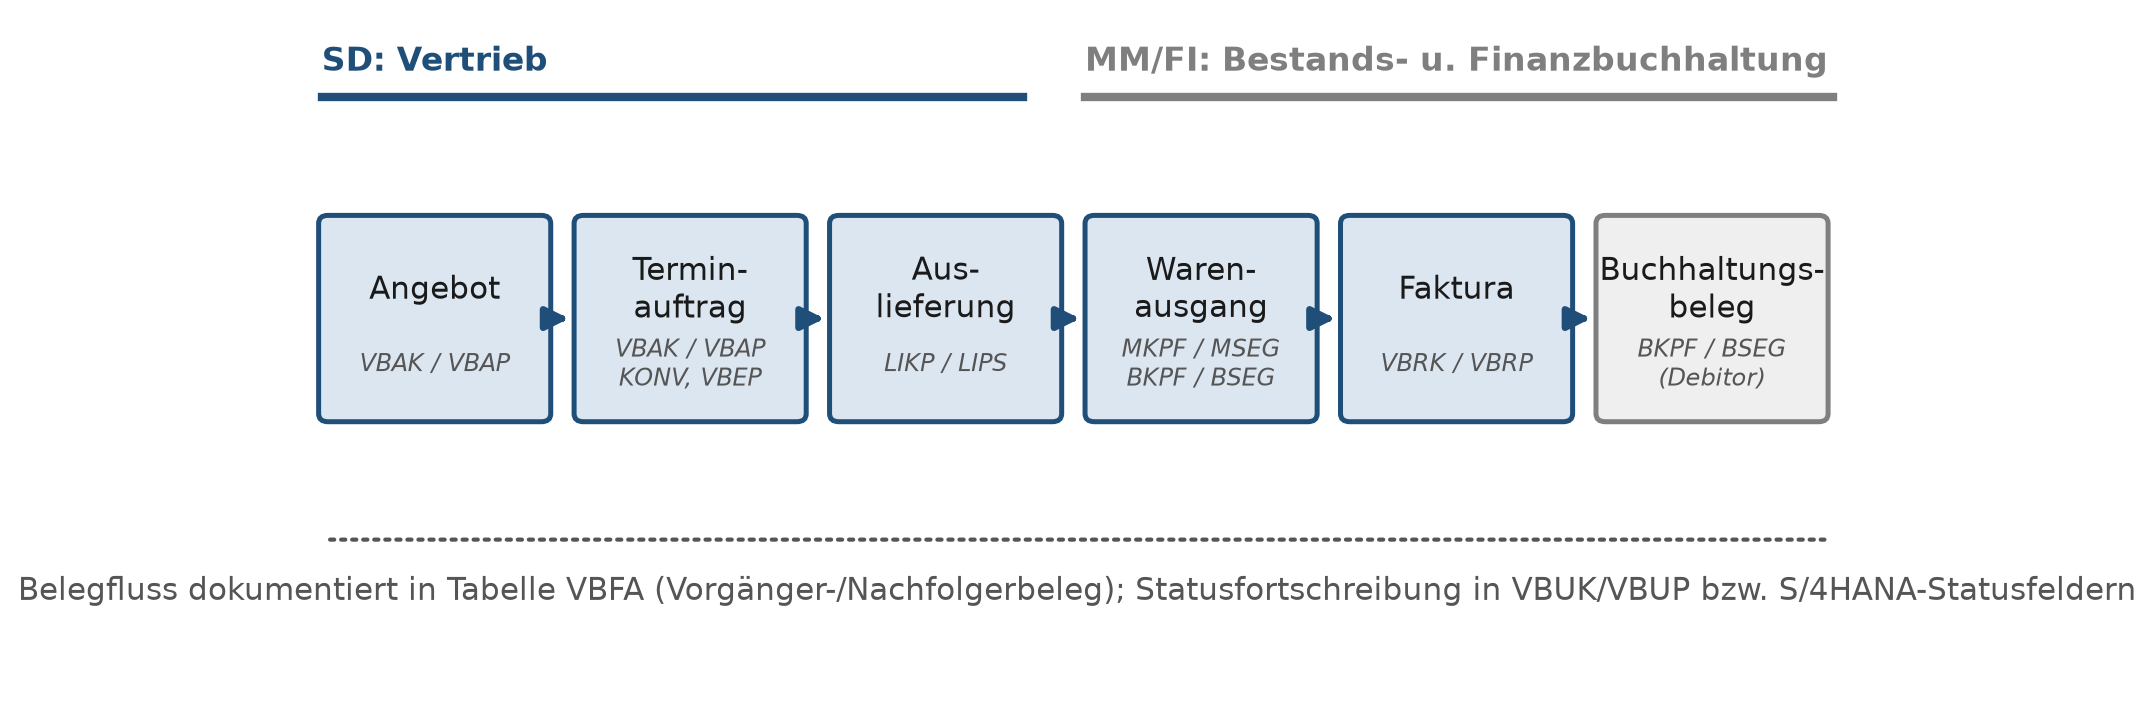
\includegraphics[width=\textwidth,height=0.36\textheight,keepaspectratio]{figures/image2.png}
\caption{\gls{sap}-Belegfluss des \gls{o2c}-Prozesses mit den zugehörigen Tabellen (Quelle: eigene Darstellung)}\label{fig:sap-belegfluss}
\end{figure}

Der eigentliche Prozess ist reicher als die reine Soll-Kette, denn an mehreren Stellen sieht der Standard Prüfungen und mögliche Sperren vor: Die Kreditprüfung kann einen Auftrag sperren, bis er freigegeben wird, die Unvollständigkeits- und Verfügbarkeitsprüfung kann die Lieferung verzögern, und Preisabweichungen können eine Fakturasperre auslösen. Ob diese Prüfungen automatisiert oder manuell, streng oder locker eingestellt sind, ist eine Frage des Customizings und damit genau der Stellhebel, an dem die Verbesserungsmaßnahmen in Kapitel~\ref{ch:anpassung} ansetzen. Ergänzend trägt jeder Beleg einen Belegtyp und einen Status (Gesamtbearbeitungs-, Liefer-, Warenausgangs- und Fakturastatus): Der Belegtyp bestimmt die zulässigen Folgebelege, der Status dokumentiert den Fortschritt und ist damit eine zum Belegfluss komplementäre Ereignisquelle für das Process Mining.

\section{Stamm- und Bewegungsdaten im \gls{sap}-Prozess}\label{sec:stamm-bewegungsdaten-sap}

\gls{sap} bildet ein Unternehmen über eine Hierarchie von Organisationseinheiten ab. An der Spitze steht der Mandant als betriebswirtschaftlich größte organisatorische Einheit, darunter der Buchungskreis als kleinste Einheit, für die eine vollständige, in sich abgeschlossene Buchhaltung geführt werden kann \parencites[Folien~357 ff.]{coletta2026_0206}[Folien~484 ff.]{coletta2026_1407}. Organisatorisch wird der Vertrieb über die Einheiten Verkaufsorganisation, Vertriebsweg und Sparte strukturiert, die zusammen den Vertriebsbereich bilden. Die Versandstelle bündelt die Versandaktivitäten für ein oder mehrere Werke \parencites[Folie~492, 520 f.]{coletta2026_1407}[Folie~398]{coletta2026_0906}. Diese Organisationsdaten sind für Process Mining nicht nur Kontext, sondern ein wertvolles Filterkriterium, weil sie den Vergleich von Prozessvarianten je Verkaufsorganisation oder Versandstelle erlauben. Der Kundenstamm wird in \gls{s/4hana} als Geschäftspartner geführt und gliedert sich in mandantenweite allgemeine Daten, Buchungskreisdaten der Finanzbuchhaltung und Vertriebsbereichsdaten \parencite[Folie~492, 502, 520 f.]{coletta2026_1407}. Der Materialstamm ist die „zentrale Quelle zum Abruf materialspezifischer Daten“ und in funktionale Sichten gegliedert \parencite[Folie~499 ff.]{coletta2026_1407}. Gerade die Vertriebsbereichsdaten des Kundenstamms, etwa Versandbedingungen und Incoterms, sind es, deren Lückenhaftigkeit im Ist-Prozess die Liefersperren (K3) auslöst. Ähnlich verhält es sich mit dem Konditionsstamm: Sind Sonderpreise dort nicht hinterlegt, weichen die Sachbearbeiter auf manuelle Eingaben im Auftrag aus, was die Fakturasperren (K5) nach sich zieht. Die Qualität der Stammdaten bestimmt somit unmittelbar, wie viele Fälle den störungsfreien Pfad verlassen, und ist damit der zentrale Ansatzpunkt jeder nachhaltigen Verbesserung.

Die Bewegungsdaten liegen in relationalen Tabellenpaaren aus Kopf- und Positionsdaten (Tabelle~\ref{tab:zentrale-sap-tabellen}). Drei Eigenschaften sind für die vorliegende Fragestellung entscheidend. Erstens trägt jeder Beleg Zeitstempel und Benutzerkennung (z.\,B. \gls{erdat}/\gls{erzet}/\gls{ernam}), sodass Ereigniszeitpunkte rekonstruierbar sind. Zweitens dokumentiert die Belegflusstabelle \gls{vbfa} jede Vorgänger-Nachfolger-Beziehung zwischen Belegen und verknüpft damit die Prozessschritte eines Falls. Drittens protokollieren Änderungsbelege (\gls{cdhdr}/\gls{cdpos}) jede nachträgliche Änderung an Belegen und Stammdaten einschließlich Datum, Uhrzeit, Benutzer und geändertem Feld. Über sie werden auch das Setzen und Lösen von Kredit-, Liefer- und Fakturasperren sichtbar \parencites[S.~63 ff.]{scheibler2021vertrieb}[Folie~375]{coletta2026_0206}. Technisch liegen alle genannten Tabellen in \gls{s/4hana} auf der spaltenorientierten In-Memory-Datenbank \gls{sap} HANA, was Massenauswertungen direkt auf den Bewegungsdaten beschleunigt \parencite[Folie~266]{coletta2026_1905}. Besonders die Änderungsbelege sind für die vorliegende Fragestellung wertvoll, weil sie Zustandsübergänge festhalten, die in den reinen Belegtabellen unsichtbar blieben: Ob und wann eine Kreditsperre gesetzt und wieder gelöst wurde, ergibt sich erst aus der Historie des Feldes \gls{cmgst} in \gls{cdpos}. Ohne diese Protokollierung wären die Sperrenmuster K2, K3 und K5 aus den Daten nicht rekonstruierbar; sie sind der Grund, warum ein Event-Log deutlich mehr Aktivitäten enthalten kann als der reine Belegfluss nahelegt.

\begin{table}[!htb]
\centering
\caption{Zentrale \gls{sap}-Tabellen des \gls{o2c}-Prozesses (Auswahl)}\label{tab:zentrale-sap-tabellen}
\small
\begin{tabularx}{\textwidth}{@{}>{\RaggedRight\arraybackslash}p{2.5cm} >{\RaggedRight\arraybackslash}p{4.4cm} Y@{}}
\toprule
\textbf{Beleg /\allowbreak{} Objekt} & \textbf{Kopf-/\allowbreak{}Positionstabelle} & \textbf{Für Process Mining relevante Felder} \\
\midrule
Kundenauftrag & \gls{vbak} /\allowbreak{} \gls{vbap} & VBELN, POSNR, \gls{erdat}/\allowbreak{}\gls{erzet}/\allowbreak{}\gls{ernam}, AUART, NETWR, \gls{lifsk}, \gls{cmgst} \\
Auslieferung & \gls{likp} /\allowbreak{} \gls{lips} & VBELN, \gls{erdat}/\allowbreak{}\gls{erzet}, \gls{lfdat}, WADAT\_IST (tatsächl. Warenausgang) \\
Faktura & \gls{vbrk} /\allowbreak{} \gls{vbrp} & VBELN, \gls{erdat}/\allowbreak{}\gls{erzet}, FKDAT, \gls{fksto}, NETWR \\
Buchhaltungsbeleg & \gls{bkpf} /\allowbreak{} \gls{bseg} (ACDOCA) & BELNR, BUDAT, \gls{augdt} \\
Belegfluss & \gls{vbfa} & VBELV/\allowbreak{}POSNV $\rightarrow$ VBELN/\allowbreak{}POSNN, VBTYP\_N, \gls{erdat}/\allowbreak{}\gls{erzet} \\
Änderungsbelege & \gls{cdhdr} /\allowbreak{} \gls{cdpos} & OBJECTCLAS (z. B. VERKBELEG), UDATE/\allowbreak{}UTIME, USERNAME, TABNAME, FNAME, Alt-/\allowbreak{}Neuwert \\
\bottomrule
\end{tabularx}
\end{table}


\section{Schnittpunkte mit anderen \gls{sap}-Modulen}\label{sec:modulschnittstellen}

Der \gls{o2c}-Prozess ist kein reiner \gls{sd}-Prozess, sondern lebt von der Integration (Tabelle~\ref{tab:modulschnittstellen}). Die Verfügbarkeitsprüfung und die Warenausgangsbuchung greifen auf die Bestandsführung des Moduls \gls{mm} zu, kundenauftragsbezogene Fertigungsaufträge entstehen im Modul \gls{pp}, die Faktura erzeugt den Buchhaltungsbeleg und den offenen Posten in \gls{fi}, das Kreditmanagement bewertet den Debitor aus \gls{fi}-Daten, und die Ergebnisrechnung im \gls{co} übernimmt Erlöse und Kosten je Marktsegment.

\begin{table}[!htb]
\centering
\caption{Schnittstellen des \gls{o2c}-Prozesses zu anderen \gls{sap}-Modulen}\label{tab:modulschnittstellen}
\small
\begin{tabularx}{\textwidth}{@{}>{\RaggedRight\arraybackslash}p{3.6cm} >{\RaggedRight\arraybackslash}p{2.8cm} Y@{}}
\toprule
\textbf{\gls{o2c}-Schritt} & \textbf{beteiligtes Modul} & \textbf{ausgetauschtes Datenobjekt /\allowbreak{} Wirkung} \\
\midrule
Verfügbarkeitsprüfung (ATP) & \gls{mm} (ggf. \gls{pp}) & Bestands-/\allowbreak{}Bedarfsabgleich; bei Fehlbestand Anstoß von Beschaffung oder Fertigung \\
Warenausgang buchen & \gls{mm} /\allowbreak{} \gls{fi} & Materialbeleg mindert Bestand; Buchungsbeleg bucht Warenaufwand \\
Faktura erstellen & \gls{fi} & debitorischer offener Posten (Forderung) wird erzeugt \\
Kreditprüfung & \gls{fi} (\gls{fscm}) & Bewertung des Debitors anhand Kreditlimit und offener Posten \\
Erlös-/Kostenzuordnung & \gls{co} & Übernahme von Erlösen und Kosten in die Ergebnisrechnung \\
\bottomrule
\end{tabularx}
\end{table}

Diese Integration über eine gemeinsame Datenhaltung ist ein Grundprinzip von \gls{erp}-Systemen \parencite[Folie~44 und 63]{coletta2026_0303} und der Grund, warum sich gerade \gls{erp}-Systeme für Process Mining eignen. Weil Informationssilos aufgebrochen und Teilprozesse miteinander verbunden sind \parencite[Folie~74]{coletta2026_1003}, hinterlässt ein Geschäftsfall seine vollständige Spur in einem einzigen System, vom Auftrag bis zum Zahlungseingang. Dass jeder Schritt dabei unmittelbar auf Bestand und Buchhaltung durchschlägt, zeigt \gls{sap} auch in eigenen Schulungsunterlagen, dort am Beispiel von \gls{sap} Business One \parencite[S.~2]{sap2013tb1000}.

Für die Analyse folgt daraus eine praktische Konsequenz: Ein vollständiges Bild des \gls{o2c}-Prozesses erfordert Daten aus mehreren Modulen. Die reinen Vertriebsbelege zeigen den Auftrag und die Rechnung, nicht aber die Bestandsbuchung im \gls{mm} oder den Zahlungsausgleich im \gls{fi}. Erst die modulübergreifende Extraktion, die \gls{sap} über die gemeinsame Datenbank technisch ermöglicht, erlaubt es, den Prozess lückenlos vom Auftrag bis zum Geldeingang abzubilden.

\chapter{Handlungsempfehlungen}\label{ch:empfehlungen}


\section{Anpassung der Unternehmensprozesse}\label{sec:anpassung-unternehmensprozesse}

Die in Kapitel~\ref{sec:gaps-auswirkungen} quantifizierten Gaps wurden zwar simulativ erzeugt, entsprechen aber Konfigurations- und Organisationsmustern, wie sie in Praxisberichten zu \gls{sap}-Anwender\-unternehmen wiederkehrend beschrieben werden\footcites(Vgl.)()[S.~3 ff.]{reinkemeyer2020processmining}[S.~21 ff.]{peters2019processmining}. Dieses Kapitel leitet ab, wie ein Unternehmen die gemessenen Ineffizienzen beheben kann, gegliedert nach organisatorischen Maßnahmen, Customizing und Erweiterungen.

Auf organisatorischer Ebene setzen drei Maßnahmen an den Wurzeln der Muster an. Erstens eine Stammdaten-Governance. Für Kundenstammdaten werden Pflichtattribute, Verantwortlichkeiten und ein Bereinigungsprojekt definiert. Das Projekt identifiziert und klassifiziert die Datenquellen, bereinigt die Bestände und überwacht die Qualität kontinuierlich. Vollständige Versanddaten und Incoterms entziehen den Liefersperren (G3) die Grundlage. Zweitens die Entlastung der Auftragserfassung, etwa durch elektronischen Datenaustausch mit den umsatzstärksten Kunden. Das reduziert Erfassungsfehler und damit die Änderungsschleife (G2). Drittens ein definierter Reklamationsprozess mit Rollen und Fristen, der die Gutschrifts- und Nachlieferungsfälle (G6) aus der informellen E-Mail-Bearbeitung in einen messbaren Ablauf überführt. Dass Stammdatenmängel der zentrale Engpasstreiber im \gls{o2c}-Prozess sind, bestätigt die Fallstudie von Adolfsson/Saleh, in der fehlerhafte Kundenstammdaten bei einem Kunden in allen Fällen manuelle Lieferterminänderungen und in rund einem Fünftel nachträgliche Preiskorrekturen erzwangen\footcite[Vgl.][S.~55 f.\ und 61]{adolfsson2026o2c}. Automatisierung, Datenintegration und fortgeschrittene Analytik gelten in der Literatur übergreifend als zentrale Hebel zur Verbesserung des \gls{o2c}-Prozesses in \gls{sap} \gls{sd}\footcite[Vgl.][S.~110 ff.]{nadukuru2024o2c}. Diese organisatorischen Maßnahmen sind Voraussetzung dafür, dass die anschließenden Systemeinstellungen überhaupt greifen. Eine automatisierte Kreditprüfung ist nur so gut wie die zugrunde liegenden Kreditstammdaten, und eine Pflichtfeldsteuerung für Versanddaten verhindert Liefersperren nur dann, wenn zugleich definiert ist, wer die fehlenden Attribute in welcher Frist pflegt. Organisatorische und technische Maßnahmen bilden also keine Alternative, sondern greifen ineinander. Praktisch beginnt eine Stammdaten-Governance mit der Benennung von Verantwortlichen je Datenobjekt, der Definition verbindlicher Pflichtfelder und Pflegestandards sowie einem einmaligen Bereinigungslauf, der Dubletten und veraltete Einträge entfernt. Erst danach greifen die Pflichtfeldprüfungen im System, ohne den laufenden Betrieb zu blockieren.

\section{Customizing im \gls{sap}-System}\label{sec:customizing}

Der Großteil der Gaps lässt sich ohne Programmierung im Customizing schließen, Tabelle~\ref{tab:massnahmenkatalog} ordnet jedem Gap die Maßnahme und den \gls{sap}-Bezug zu. Kern ist die Automatisierung der Kreditprüfung im \gls{sap} Credit Management. Bestandskunden mit gutem Zahlungsverhalten erhalten regelbasierte Scores und Limits, sodass Sperren nur noch bei tatsächlichen Risikofällen entstehen (G1). Die Unvollständigkeitsprüfung und Pflichtfeldsteuerung verhindert Aufträge mit fehlenden Versanddaten (G3), die Umstellung des Fakturavorrats auf tägliche Läufe beseitigt die künstliche Wartezeit vor der Rechnungsstellung (G4), und ein restriktives Berechtigungskonzept für manuelle Preisänderungen erzwingt die Pflege im Konditionsstamm (G5). Nachträgliche Auftragsänderungen (G2) werden durch eine entlastete, fehlerärmere Auftragserfassung gesenkt, insbesondere durch die \gls{edi}-Anbindung der umsatzstärksten Kunden (M6)\footcite[Vgl.][S.~110 ff.]{nadukuru2024o2c}.

\begin{table}[!htb]
\centering
\caption{Maßnahmenkatalog mit Gaps, Lösungsansätzen und \gls{sap}-Bezug}\label{tab:massnahmenkatalog}
\small
\begin{tabularx}{\textwidth}{@{}>{\RaggedRight\arraybackslash}p{3.0cm} >{\RaggedRight\arraybackslash}p{2.8cm} >{\RaggedRight\arraybackslash}p{4.4cm} >{\RaggedRight\arraybackslash}p{3.9cm}@{}}
\toprule
\textbf{Maßnahme} & \textbf{Typ} & \textbf{\gls{sap}-Bezug} & \textbf{Adressiertes Gap /\allowbreak{} erwarteter Effekt} \\
\midrule
M1 Automatisierte Kreditprüfung & Customizing & \gls{sap} Credit Management: Scoring-Regeln, Limitprofile, Ausnahmeliste & G1: Sperrquote von 34,1 \% deutlich reduziert; Median-Liegezeit 1,9 AT entfällt für Bestandskunden \\
M2 Stammdatenbereinigung u. Pflichtfelder & organisatorisch + Customizing & Unvollständigkeitsprüfung, Pflichtfeldsteuerung, Geschäftspartnerpflege & G3: Liefersperrenquote von 12,3 \% Richtung Restrisiko; 3,9 $\rightarrow$ 0,8 AT bis Lieferbeleg \\
M3 Tägliche Fakturierungsläufe & Customizing & Fakturavorrat (VF04/\allowbreak{}VF06) als täglicher Hintergrundjob & G4: Liegezeit WA $\rightarrow$ Faktura von 2,6 auf ca. 0,5 AT \\
M4 Konditionspflege u. Berechtigungen & Customizing + organisatorisch & Preisfindung/\allowbreak{}Konditionstechnik, Rollenkonzept & G5: Fakturasperren (7,9 \%) weitgehend vermieden \\
M5 Workflow Reklamation/\allowbreak{}Gutschrift & Customizing/\allowbreak{}Workflow & Freigabeworkflow für Gutschriftsanforderungen & G6: definierte Durchlaufzeit, Transparenz \\
M6 \gls{edi}-Anbindung Top-Kunden & Erweiterung & \gls{idoc}-Eingang für Bestellungen (ORDERS) & G2: Änderungsquote (22,7 \%) sinkt; weniger Erfassungsfehler \\
\bottomrule
\end{tabularx}
\end{table}

Am Beispiel der Kreditprüfung (M1) lässt sich der Hebel konkretisieren. Im Ist-Zustand wird jeder Auftrag, der ein statisches Kreditlimit überschreitet, gesperrt und manuell freigegeben, unabhängig vom tatsächlichen Risiko. Das \gls{sap} Credit Management ordnet Kunden stattdessen Risikoklassen mit eigenen Prüfregeln und Limits zu, sodass Bestandskunden mit tadellosem Zahlungsverhalten automatisch freigegeben werden, während echte Risikofälle weiterhin geprüft werden. Die Sperre wird damit vom Regelfall zur Ausnahme, ohne den Schutz vor Forderungsausfällen aufzugeben. Zu beachten ist, dass mehrere Maßnahmen ineinandergreifen. M1 setzt gepflegte Kreditstammdaten voraus und der Verzicht auf manuelle Preise (M4) einen vollständigen Konditionsstamm. Die Stammdaten-Governance aus Kapitel~\ref{sec:anpassung-unternehmensprozesse} ist damit nicht eine Maßnahme unter mehreren, sondern das Fundament, auf dem die technischen Anpassungen aufbauen.

Über die Kreditprüfung hinaus greifen die übrigen Customizing-Maßnahmen an klar umrissenen Konfigurationspunkten an. Die Unvollständigkeitsprüfung wird so eingestellt, dass ein Auftrag ohne gepflegte Versanddaten gar nicht erst zur Lieferung freigegeben wird, was die Liefersperren an der Wurzel verhindert. Der Fakturavorrat wird von einem wöchentlichen auf einen täglichen Hintergrundjob umgestellt, und die Berechtigung, Preise manuell im Auftrag zu überschreiben, wird auf wenige Rollen beschränkt, sodass Sonderkonditionen künftig im Konditionsstamm gepflegt werden. Keine dieser Einstellungen erfordert eine Programmierung, sie nutzen ausschließlich vorgesehene Parameter des Standards, was Wartbarkeit und Release-Fähigkeit erhält.

\section{Erweiterungen und kontinuierliches Monitoring}\label{sec:modifikationen-monitoring}

Eigenentwicklungen oder Modifikationen des \gls{sap}-Standards sind für keines der sechs Gaps erforderlich, im Einklang mit dem bewährten Grundsatz möglichst großer Standardnähe. Als Erweiterung im Sinne des Enhancement-Typs des Process Mining empfiehlt sich jedoch ein kontinuierliches Prozessmonitoring. Die Extraktionslogik aus Kapitel~\ref{sec:logkonstruktion} wird als wiederkehrender Ladeprozess eingerichtet, sodass Kennzahlen wie Sperrquoten, Liegezeiten und Happy-Path-Anteil laufend überwacht und Maßnahmenwirkungen gemessen werden können. Process Mining wandelt sich damit von einer einmaligen Diagnose zu einem dauerhaften Steuerungsinstrument\footcite[Vgl.][S.~3 ff.]{reinkemeyer2020processmining}. Die verwendete Werkzeugkette aus Python und \gls{pm4py} zeigt, dass dafür nicht zwingend eine kommerzielle Plattform erforderlich ist, wie sie \gls{sap} mit dem Beispielinhalt „Process Mining on \gls{sap} \gls{s/4hana}“ in \gls{papm} für dasselbe Szenario anbietet\footcite[Vgl.][Abschnitt~2.1, S.~9]{sap2022samplecontent}.

Der Aufbau eines solchen Monitorings ist selbst ein kleines Datenprojekt. Die Extraktion muss regelmäßig und möglichst inkrementell erfolgen, die Kennzahlen sind in einem Dashboard zu verdichten, und für kritische Größen wie eine wieder steigende Sperrquote sind Schwellenwerte für Warnungen festzulegen. Damit wird aus der einmaligen Fit/Gap-Analyse ein geschlossener Regelkreis, in dem Abweichungen früh erkannt und gegengesteuert werden, bevor sie sich in Durchlaufzeit und Forderungslaufzeit niederschlagen. Konkret bieten sich als Kennzahlen die bereits in der Analyse verwendeten Größen an, also die Sperrquoten je Sperrentyp, die Median-Liegezeiten je Prozessübergang, der Anteil konformer Fälle und die Durchlaufzeit bis zur Faktura. Werden sie zusätzlich je Verkaufsorganisation oder Kundengruppe aufgeschlüsselt, lassen sich Problembereiche gezielt eingrenzen, statt nur einen Gesamtdurchschnitt zu betrachten.

\section{Implementierungsstrategie}\label{sec:schrittweise-umsetzung}

Die Umsetzung der Maßnahmen wird in die etablierten Phasen einer \gls{erp}-Anpassung gegliedert. Diese umfassen Projektplanung, Systemkonfiguration, Datenbereinigung, Testphase, Schulung und Go-Live. Insgesamt ist sie auf sechs Monate ausgelegt (Abbildung~\ref{fig:implementierungsplan}). Nach dem Detailkonzept (P1) laufen die Stammdatenbereinigung (P2) und das Customizing des Kreditmanagements (P3) parallel. Die Umstellung der Fakturierungsläufe (P4) ist bewusst früh terminiert, weil sie mit geringem Aufwand die größte Liquiditätswirkung entfaltet („Quick Win“, Abbildung~\ref{fig:liegezeiten}). Es folgen der Gutschriften-Workflow (P5), Integrationstests und Schulungen (P6) sowie Go-Live mit Hypercare-Phase (P7). Die Planung nutzt die klassischen Instrumente Projektstrukturplan, Meilensteine und Gantt-Diagramm.

\begin{figure}[!htb]
\centering
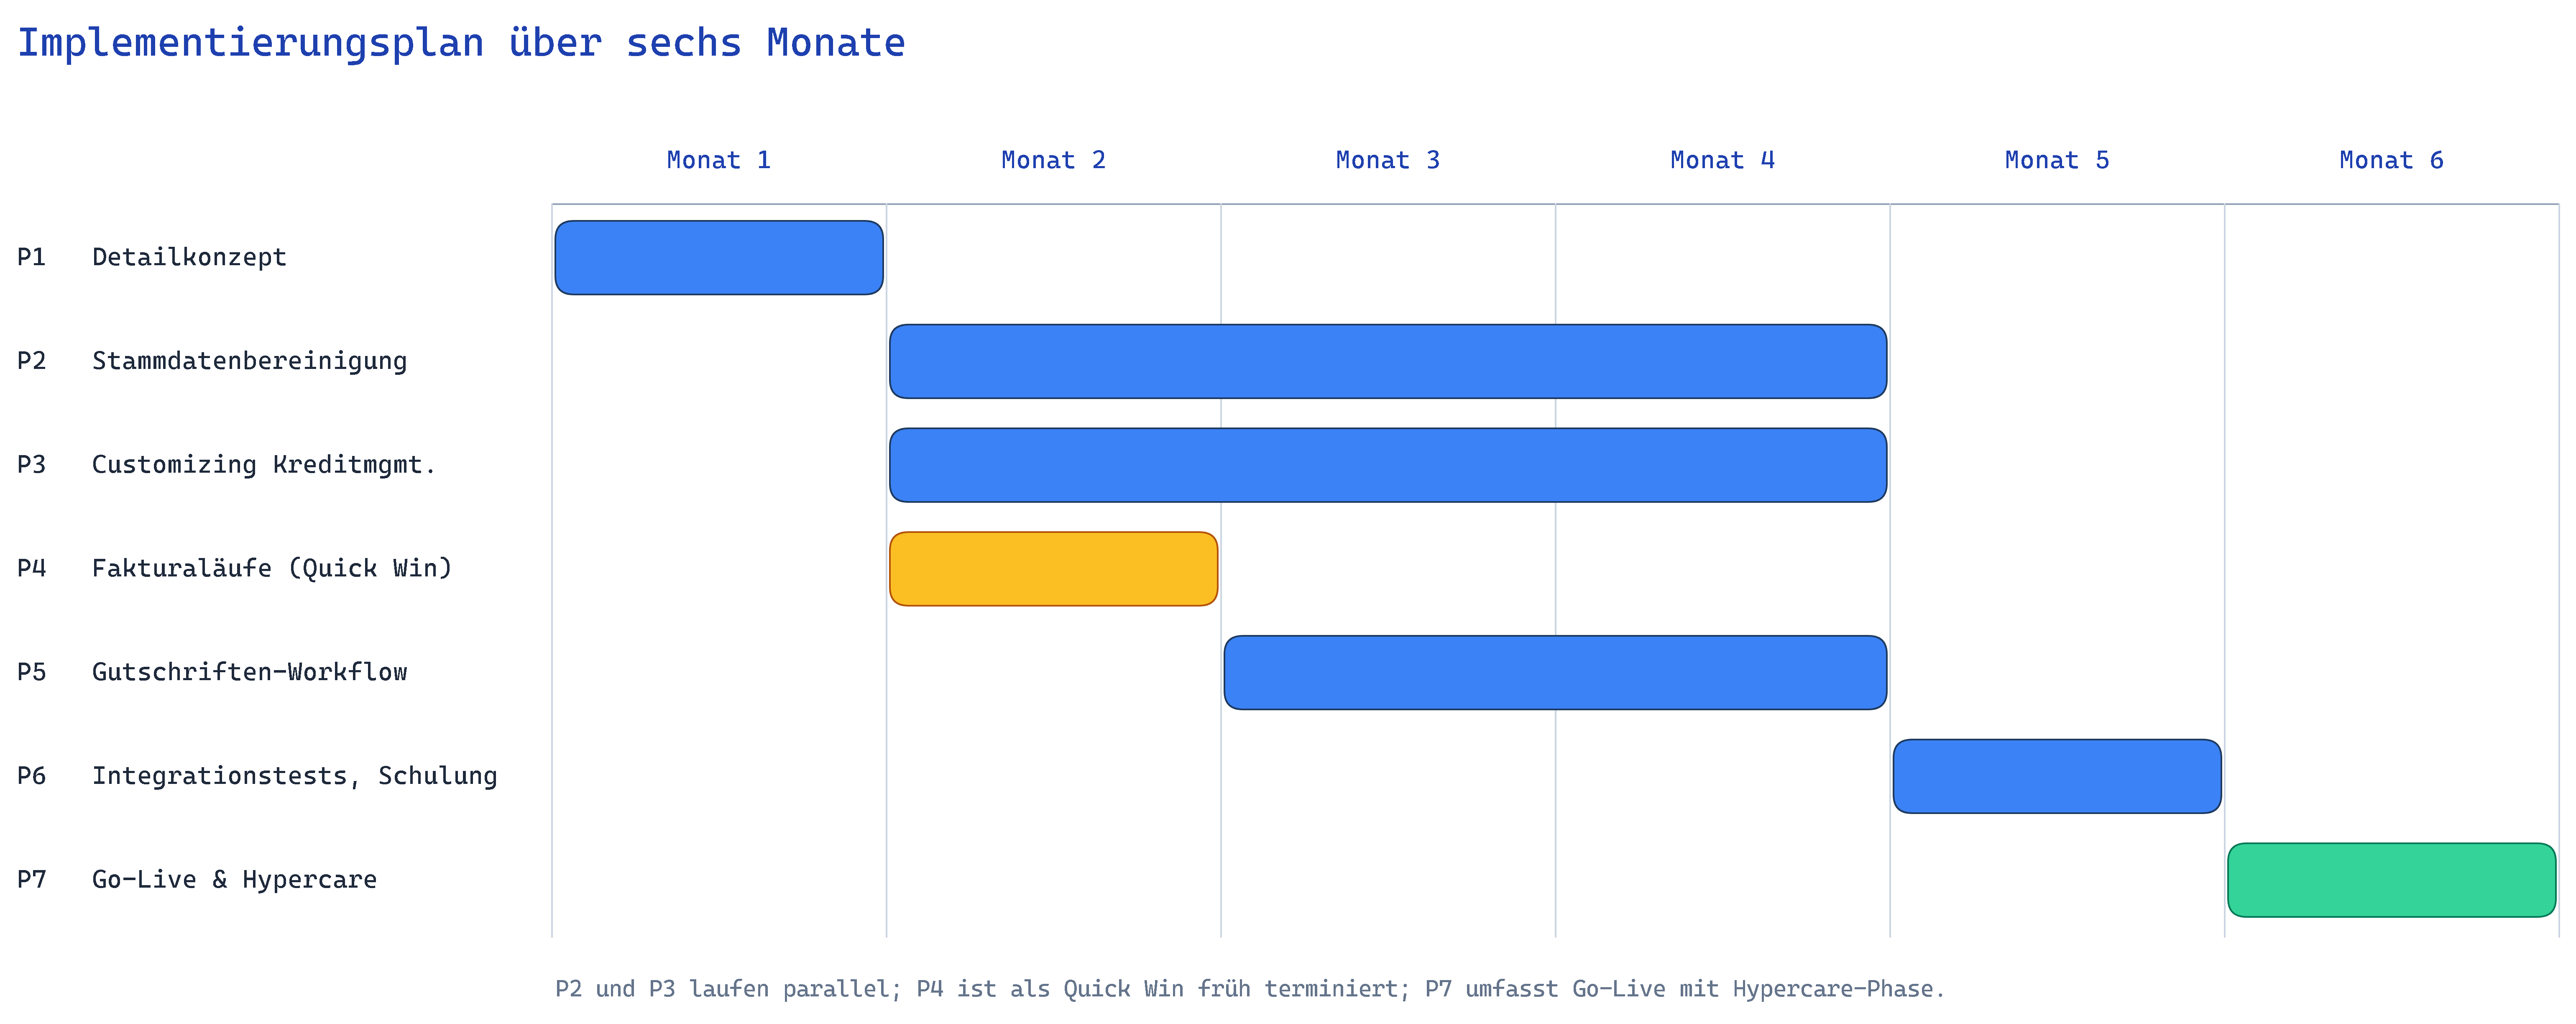
\includegraphics[width=\textwidth,height=0.36\textheight,keepaspectratio]{figures/image7.png}
\caption{Implementierungsplan über sechs Monate}\label{fig:implementierungsplan}
\end{figure}

Ein iteratives, phasenweises Vorgehen ist auch aus Risikosicht geboten. Statt alle sechs Maßnahmen gleichzeitig produktiv zu setzen, werden sie nacheinander eingeführt und ihre Wirkung jeweils über das Prozessmonitoring gemessen, bevor die nächste folgt. So lässt sich etwa bei der automatisierten Kreditprüfung (M1) in einem Parallellauf beobachten, ob die neuen Regeln zu viele Aufträge blockieren oder umgekehrt Risikofälle durchlassen, und die Schwellenwerte können nachjustiert werden, bevor die manuelle Prüfung vollständig abgelöst wird. Dieses Vorgehen entspricht einem Phased Rollout und reduziert das Risiko, dass eine fehlerhafte Einstellung den gesamten \gls{o2c}-Prozess stört. Inhaltlich gliedert sich das Vorhaben damit in eine Vorbereitungsphase (Detailkonzept und Priorisierung anhand der gemessenen Kennzahlen), eine Umsetzungsphase (parallele Stammdatenbereinigung und Customizing mit dem Fakturalauf als frühem Quick Win) und eine Stabilisierungsphase (Integrationstest, Schulung, Go-Live und Hypercare). Der Übergang von einer Phase zur nächsten ist jeweils an ein messbares Ergebnis geknüpft, etwa eine gesunkene Sperrquote im Parallellauf. Die Gesamtdauer von sechs Monaten ergibt sich dabei weniger aus dem technischen Aufwand der einzelnen Einstellungen, der überschaubar ist, als aus der Stammdatenbereinigung, den Testzyklen und der notwendigen Eingewöhnung der Anwender.

Für die Testphase sind Integrations-, User-Acceptance- und Regressionstests mit realistischen Testdaten vorgesehen. Personell erfordert das Vorhaben eine interne Projektleitung (ca. 0,3 \gls{vzae}), je einen Key-User aus Vertrieb, Versand und Debitorenbuchhaltung (je ca. 0,2 \gls{vzae}), externe \gls{sd}-/\gls{fscm}-Beratung (ca. 25 Personentage) sowie die \gls{it} für Berechtigungen und Hintergrundjobs. Die externen Kosten lassen sich auf Basis marktüblicher Beratungstagessätze grob auf 60.000 bis 80.000 \euro{} schätzen. Dem stehen im modellierten Szenario rund 1.950 eingesparte Klärungsstunden pro Jahr (ca. 1,2 \gls{vzae}) sowie eine um mehrere Tage verkürzte Zeitspanne bis zur Rechnungsstellung gegenüber, die die Forderungslaufzeit unmittelbar senkt. Nach der \gls{roi}-Logik amortisiert sich das Vorhaben unter diesen Annahmen bereits im ersten Jahr. Nach dem Go-Live werden Erfolgskriterien als Post-Go-Live-Metriken definiert und in der Hypercare-Phase proaktiv überwacht, unmittelbar über das Prozessmonitoring aus Kapitel~\ref{sec:modifikationen-monitoring} mit den Kennzahlen aus Anhang III.

Die Testphase verdient dabei besondere Aufmerksamkeit, weil die Maßnahmen tief in den erlöswirksamen Prozess eingreifen. Neben den funktionalen Integrationstests sind Regressionstests der angrenzenden Prozesse in Beschaffung, Bestandsführung und Debitorenbuchhaltung vorzusehen, und die neuen Kreditregeln sind an einem repräsentativen Ausschnitt historischer Aufträge zu erproben, um Fehlsperren zu vermeiden. Erst nach erfolgreichem User-Acceptance-Test durch die Key-User erfolgt der Go-Live.

Wirtschaftlich ist das Vorhaben auch unter konservativen Annahmen tragfähig. Den einmaligen externen Kosten stehen wiederkehrende Effekte gegenüber, nämlich eingesparte Klärungsstunden, eine kürzere Forderungslaufzeit und eine höhere Liefertermintreue. Weil die Liquiditätswirkung der täglichen Fakturierung sofort und ohne laufende Kosten eintritt, während die Beratungskosten nur einmalig anfallen, verschiebt sich das Kosten-Nutzen-Verhältnis bereits im ersten Jahr deutlich ins Positive. Entscheidend für die Belastbarkeit dieser Rechnung ist, dass die zugrunde liegenden Ist-Werte aus der Analyse gemessen und nicht geschätzt sind, sodass die erwarteten Einsparungen an konkreten, nachprüfbaren Kennzahlen festgemacht werden können.

\section{Risiken und Veränderungsmanagement}\label{sec:risikobewertung}

Die Risiken des Vorhabens liegen weniger in der Technik als in Datenqualität, Organisation und Akzeptanz. Tabelle~\ref{tab:risikomatrix} bewertet die wichtigsten Risiken und hinterlegt Gegenmaßnahmen. Hervorzuheben ist das Datenschutzrisiko, das beim Übergang von synthetischen auf reale Event-Logs entsteht. Reale Logs enthalten Benutzerkennungen und erlauben Leistungs- und Verhaltensauswertungen, Betriebsrat und Datenschutzbeauftragte sind daher früh einzubinden, und die Analysen sind auf pseudonymisierte, nicht personenbezogene Auswertungen zu beschränken.

\begin{table}[!htb]
\centering
\caption{Risikomatrix der Implementierung}\label{tab:risikomatrix}
\small
\begin{tabularx}{\textwidth}{@{}Y l l Y@{}}
\toprule
\textbf{Risiko} & \textbf{Eintritt} & \textbf{Auswirkung} & \textbf{Gegenmaßnahme} \\
\midrule
Datenqualität schlechter als angenommen (Stammdaten) & hoch & mittel & frühe Testextraktion, Bereinigung priorisieren, Puffer in P2 \\
Zu scharfe Kreditregeln blockieren Aufträge /\allowbreak{} zu laxe erhöhen Forderungsausfälle & mittel & hoch & Pilotbetrieb mit Parallellauf, Schwellenwerte iterativ justieren, Ausnahmeliste \\
Akzeptanz: Mitarbeitende fühlen sich durch Prozessdaten überwacht (reale Logs) & mittel & hoch & Pseudonymisierung, Betriebsvereinbarung, transparente Kommunikation der Ziele \\
Scope-Ausweitung (weitere Prozesse „auch noch schnell“) & mittel & mittel & Change-Request-Verfahren, Priorisierung nach Nutzwert \\
Wissensabfluss nach Beratungsende & niedrig & mittel & Dokumentation, Key-User-Schulung, Betreuungsvereinbarung \\
\bottomrule
\end{tabularx}
\end{table}

Neben diesen sachlichen Risiken ist das Veränderungsmanagement entscheidend, weil die Maßnahmen etablierte Arbeitsweisen ablösen. Die Umstellung von der manuellen auf die automatisierte Kreditfreigabe etwa entzieht der Debitorenbuchhaltung eine gewohnte Kontrollaufgabe und muss durch frühzeitige Einbindung, transparente Kommunikation der Ziele und Schulung begleitet werden. Gerade weil Process Mining das tatsächliche Verhalten sichtbar macht, ist der offene Umgang mit den Ergebnissen, verbunden mit der klaren Zusage, die Auswertung nicht zur individuellen Leistungskontrolle zu nutzen, eine Voraussetzung für die Akzeptanz im Team.

\section{Erfahrungen und Empfehlungen für vergleichbare Projekte}\label{sec:erkenntnisse-empfehlungen}

Die Datenaufbereitung erwies sich als der eigentliche Engpass, selbst bei synthetischen Daten. In einer ersten Fassung des Simulationsmodells erzeugten nicht streng monotone Zeitstempel Schein-Kanten im entdeckten Modell. Solche Granularitäts- und Sortierprobleme treten auch bei realen \gls{sap}-Extraktionen auf, wenn tagesgenaue Felder wie \gls{augdt} mit sekundengenauen Zeitstempeln gemischt werden, und müssen vor der Discovery behoben werden, sonst analysiert man Artefakte statt Prozesse. Sie entsprechen den in der Literatur katalogisierten Imperfektionsmustern von Event-Logs, für die dort ein systematisches Bereinigungsvorgehen empfohlen wird\footcite[Vgl.][S.~132 ff.]{suriadi2017imperfection}. Konkret zeigte sich die Bedeutung der Datenaufbereitung daran, dass erst die Erzwingung streng monoton steigender Zeitstempel je Fall die scheinbaren Rücksprünge im Modell beseitigte. Dieses Detail wäre bei einer flüchtigen Betrachtung der Werkzeugausgabe leicht als echter Prozessschritt fehlgedeutet worden. Die Lehre daraus ist, dass die Plausibilität des Event-Logs vor jeder inhaltlichen Interpretation zu prüfen ist. Ebenso zeigte sich, dass die Methodenwahl kein akademisches Detail ist. Zwischen Alpha-Algorithmus und Inductive Miner lagen auf demselben Log deutliche Unterschiede (Fitness 0,646 gegenüber 0,996), und beim Soll-Abgleich machte erst der Wechsel vom Token-Replay zu Alignments die tatsächliche Konformität sichtbar (Kapitel~\ref{sec:gaps-auswirkungen}). Wer Werkzeugausgaben interpretiert, muss wissen, welcher Algorithmus mit welchen Parametern dahinterliegt. Eine zweite Grenze betrifft die Reichweite der Daten selbst. Ein Event-Log zeigt, \emph{was} geschehen ist, nicht \emph{warum}. In der Fallstudie von Adolfsson/Saleh blieb eine durchgängige manuelle Auftragsabstimmung mit dem Vertrieb unsichtbar, weil sie keine digitale Spur im \gls{erp}-System hinterließ\footcite[Vgl.][S.~50 und 62]{adolfsson2026o2c}. Für den synthetischen Log ist diese Grenze konstruktionsbedingt gegenstandslos, für die Übertragung auf reale Systeme jedoch zentral.

Daraus folgen vier Empfehlungen. Erstens sollten Kennzahlen wie Sperrquoten, Liegezeiten je Übergang, Happy-Path-Anteil und Zeit bis zur Faktura bereits vor der Analyse definiert werden. Ohne Ziel-\gls{kpi}s erzeugt Process Mining beeindruckende, aber folgenlose Visualisierungen. Zweitens verdient die Log-Qualitätsprüfung (Monotonie, Granularität, Vollständigkeit) einen festen Platz vor jeder Discovery. Drittens gehört beim Übergang auf reale Logs der Datenschutz an den Anfang, mit Pseudonymisierung der Benutzerkennungen und früher Einbindung von Betriebsrat und Datenschutzbeauftragten (Kapitel~\ref{sec:risikobewertung}). Viertens gilt der Grundsatz möglichst großer Standardnähe auch für die Behebung der Gaps. Alle sechs Maßnahmen kommen ohne Modifikation aus, was Wartbarkeit und Release-Fähigkeit erhält. Diese Empfehlungen decken sich mit der Praxisliteratur, die rät, Analysen breit-aggregiert zu beginnen, das Werkzeug mit Interviews und Workshops zu kombinieren und den Untersuchungsumfang zunächst eng zu fassen\footcite[Vgl.][S.~71 f.]{adolfsson2026o2c}. Eine fünfte Erkenntnis betrifft das Zusammenspiel von Methode und Fachwissen. Process Mining liefert präzise Diagnosen, aber keine Therapien. Die Entscheidung etwa, dass die Batch-Fakturierung trotz ihrer scheinbaren Harmlosigkeit die lohnendste erste Maßnahme ist, erfordert betriebswirtschaftliches Urteilsvermögen und Kenntnis des \gls{sap}-Customizings. Das datengetriebene Vorgehen ersetzt Prozessworkshops also nicht, es macht sie gezielter und beweisbarer\footcite[Vgl.][S.~71 f.]{adolfsson2026o2c}. Nicht zuletzt lohnt der Blick über den eigenen Prozess hinaus. Die Praxisliteratur und die herangezogene Fallstudie zeigen übereinstimmend, dass die größten Effekte weniger in ausgefeilteren Algorithmen als in sauberen Stammdaten und klar geschnittenen Prozessen liegen\footcites(Vgl.)()[S.~110 ff.]{nadukuru2024o2c}[S.~71 f.]{adolfsson2026o2c}. Process Mining ist damit vor allem ein Instrument, um diese unspektakulären, aber wirksamen Hebel überhaupt sichtbar und ihre Behebung messbar zu machen.

Langfristig liegt der Wert weniger in der einmaligen Diagnose als in der Verstetigung. Da Simulation und Analyse vollständig skriptbasiert und reproduzierbar sind, lässt sich dieselbe Auswertung nach jeder Prozessänderung erneut ausführen, als kontinuierliches Monitoring mit den Kennzahlen aus Anhang III (Kapitel~\ref{sec:modifikationen-monitoring}). Für die Organisation verschiebt das die Diskussionsgrundlage dauerhaft von Einzelmeinungen zu gemessener Evidenz. Prozessverbesserung wird überprüfbar und Prozessverantwortung messbar. Erfahrungsgemäß entsteht daraus ein kultureller Wandel. Wo Kennzahlen sichtbar sind, kehren alte Muster wie schleichend zunehmende manuelle Preisänderungen seltener unbemerkt zurück, weil jede Abweichung im Monitoring auffällt. Perspektivisch ist die Übertragung auf weitere Belegflüsse wie den Purchase-to-Pay-Prozess angelegt, für den der \gls{bpi}-Challenge-2019-Log als öffentliches Übungsfeld bereitsteht\footcite[Vgl.][]{vandongen2019bpi}.

\chapter{Anpassung und Lösungsansätze}\label{ch:anpassung}


\section{Vorschläge zur Anpassung der Unternehmensprozesse}\label{sec:anpassung-unternehmensprozesse}

Die in Kapitel~\ref{sec:gaps-auswirkungen} quantifizierten Gaps wurden zwar simulativ erzeugt, entsprechen aber Konfigurations- und Organisationsmustern, wie sie in Praxisberichten zu \gls{sap}-Anwender\-unternehmen wiederkehrend beschrieben werden \parencites[S.~3 ff.]{reinkemeyer2020processmining}[S.~21 ff.]{peters2019processmining}. Dieses Kapitel leitet ab, wie ein Unternehmen die gemessenen Ineffizienzen beheben kann, gegliedert nach organisatorischen Maßnahmen, Customizing und Erweiterungen.

Auf organisatorischer Ebene setzen drei Maßnahmen an den Wurzeln der Muster an. Erstens eine Stammdaten-Governance. Für Kundenstammdaten werden Pflichtattribute, Verantwortlichkeiten und ein Bereinigungsprojekt definiert, das Vorgehen orientiert sich an den bewährten Schritten der Datenmigration. Datenquellen identifizieren, klassifizieren, bereinigen und die Qualität kontinuierlich überwachen \parencite[Folie~324 ff.]{coletta2026_0206}. Vollständige Versanddaten und Incoterms entziehen den Liefersperren (G3) die Grundlage. Zweitens die Entlastung der Auftragserfassung, etwa durch elektronischen Datenaustausch mit den umsatzstärksten Kunden. Das reduziert Erfassungsfehler und damit die Änderungsschleife (G2). Drittens ein definierter Reklamationsprozess mit Rollen und Fristen, der die Gutschrifts- und Nachlieferungsfälle (G6) aus der informellen E-Mail-Bearbeitung in einen messbaren Ablauf überführt. Dass Stammdatenmängel der zentrale Engpasstreiber im \gls{o2c}-Prozess sind, bestätigt die Fallstudie von Adolfsson/Saleh, in der fehlerhafte Kundenstammdaten bei einem Kunden in allen Fällen manuelle Lieferterminänderungen und in rund einem Fünftel nachträgliche Preiskorrekturen erzwangen \parencite[S.~55 f.\ und 61]{adolfsson2026o2c}. Automatisierung, Datenintegration und fortgeschrittene Analytik gelten in der Literatur übergreifend als zentrale Hebel zur Verbesserung des \gls{o2c}-Prozesses in \gls{sap} \gls{sd} \parencite[S.~110 ff.]{nadukuru2024o2c}. Diese organisatorischen Maßnahmen sind Voraussetzung dafür, dass die anschließenden Systemeinstellungen überhaupt greifen. Eine automatisierte Kreditprüfung ist nur so gut wie die zugrunde liegenden Kreditstammdaten, und eine Pflichtfeldsteuerung für Versanddaten verhindert Liefersperren nur dann, wenn zugleich definiert ist, wer die fehlenden Attribute in welcher Frist pflegt. Organisatorische und technische Maßnahmen bilden also keine Alternative, sondern greifen ineinander. Praktisch beginnt eine Stammdaten-Governance mit der Benennung von Verantwortlichen je Datenobjekt, der Definition verbindlicher Pflichtfelder und Pflegestandards sowie einem einmaligen Bereinigungslauf, der Dubletten und veraltete Einträge entfernt; erst danach greifen die Pflichtfeldprüfungen im System, ohne den laufenden Betrieb zu blockieren.

\section{Möglichkeiten des Customizings im \gls{sap}-System}\label{sec:customizing}

Der Großteil der Gaps lässt sich ohne Programmierung im Customizing schließen, Tabelle~\ref{tab:massnahmenkatalog} ordnet jedem Gap die Maßnahme und den \gls{sap}-Bezug zu. Kern ist die Automatisierung der Kreditprüfung im \gls{sap} Credit Management. Bestandskunden mit gutem Zahlungsverhalten erhalten regelbasierte Scores und Limits, sodass Sperren nur noch bei tatsächlichen Risikofällen entstehen (G1). Die Unvollständigkeitsprüfung und Pflichtfeldsteuerung verhindert Aufträge mit fehlenden Versanddaten (G3), die Umstellung des Fakturavorrats auf tägliche Läufe beseitigt die künstliche Wartezeit vor der Rechnungsstellung (G4), und ein restriktives Berechtigungskonzept für manuelle Preisänderungen erzwingt die Pflege im Konditionsstamm (G5). Nachträgliche Auftragsänderungen (G2) werden durch eine entlastete, fehlerärmere Auftragserfassung gesenkt, insbesondere durch die \gls{edi}-Anbindung der umsatzstärksten Kunden (M6). Zu den typischen Customizing-Aktivitäten zählen dabei das Abbilden von Geschäftsprozessen, Grundeinstellungen und Berechtigungen \parencite[Folie~349]{coletta2026_0206}, Workflows für Freigaben (hier für Gutschriften) sind Teil der Systemkonfiguration \parencite[Folie~244]{coletta2026_0505}.

\begin{table}[!htb]
\centering
\caption{Maßnahmenkatalog: Gaps, Lösungsansätze und \gls{sap}-Bezug}\label{tab:massnahmenkatalog}
\small
\begin{tabularx}{\textwidth}{@{}>{\RaggedRight\arraybackslash}p{3.0cm} >{\RaggedRight\arraybackslash}p{2.8cm} >{\RaggedRight\arraybackslash}p{4.4cm} >{\RaggedRight\arraybackslash}p{3.9cm}@{}}
\toprule
\textbf{Maßnahme} & \textbf{Typ} & \textbf{\gls{sap}-Bezug} & \textbf{Adressiertes Gap /\allowbreak{} erwarteter Effekt} \\
\midrule
M1 Automatisierte Kreditprüfung & Customizing & \gls{sap} Credit Management: Scoring-Regeln, Limitprofile, Ausnahmeliste & G1: Sperrquote von 34,1 \% deutlich reduziert; Median-Liegezeit 1,9 AT entfällt für Bestandskunden \\
M2 Stammdatenbereinigung u. Pflichtfelder & organisatorisch + Customizing & Unvollständigkeitsprüfung, Pflichtfeldsteuerung, Geschäftspartnerpflege & G3: Liefersperrenquote von 12,3 \% Richtung Restrisiko; 3,9 $\rightarrow$ 0,8 AT bis Lieferbeleg \\
M3 Tägliche Fakturierungsläufe & Customizing & Fakturavorrat (VF04/\allowbreak{}VF06) als täglicher Hintergrundjob & G4: Liegezeit WA $\rightarrow$ Faktura von 2,6 auf ca. 0,5 AT \\
M4 Konditionspflege u. Berechtigungen & Customizing + organisatorisch & Preisfindung/\allowbreak{}Konditionstechnik, Rollenkonzept & G5: Fakturasperren (7,9 \%) weitgehend vermieden \\
M5 Workflow Reklamation/\allowbreak{}Gutschrift & Customizing/\allowbreak{}Workflow & Freigabeworkflow für Gutschriftsanforderungen & G6: definierte Durchlaufzeit, Transparenz \\
M6 \gls{edi}-Anbindung Top-Kunden & Erweiterung & \gls{idoc}-Eingang für Bestellungen (ORDERS) & G2: Änderungsquote (22,7 \%) sinkt; weniger Erfassungsfehler \\
\bottomrule
\end{tabularx}
\end{table}

Am Beispiel der Kreditprüfung (M1) lässt sich der Hebel konkretisieren. Im Ist-Zustand wird jeder Auftrag, der ein statisches Kreditlimit überschreitet, gesperrt und manuell freigegeben, unabhängig vom tatsächlichen Risiko. Das \gls{sap} Credit Management ordnet Kunden stattdessen Risikoklassen mit eigenen Prüfregeln und Limits zu, sodass Bestandskunden mit tadellosem Zahlungsverhalten automatisch freigegeben werden, während echte Risikofälle weiterhin geprüft werden. Die Sperre wird damit vom Regelfall zur Ausnahme, ohne den Schutz vor Forderungsausfällen aufzugeben. Zu beachten ist, dass mehrere Maßnahmen ineinandergreifen: M1 setzt gepflegte Kreditstammdaten voraus und der Verzicht auf manuelle Preise (M4) einen vollständigen Konditionsstamm. Die Stammdaten-Governance aus Kapitel~\ref{sec:anpassung-unternehmensprozesse} ist damit nicht eine Maßnahme unter mehreren, sondern das Fundament, auf dem die technischen Anpassungen aufbauen.

Über die Kreditprüfung hinaus greifen die übrigen Customizing-Maßnahmen an klar umrissenen Konfigurationspunkten an. Die Unvollständigkeitsprüfung wird so eingestellt, dass ein Auftrag ohne gepflegte Versanddaten gar nicht erst zur Lieferung freigegeben wird, was die Liefersperren an der Wurzel verhindert. Der Fakturavorrat wird von einem wöchentlichen auf einen täglichen Hintergrundjob umgestellt, und die Berechtigung, Preise manuell im Auftrag zu überschreiben, wird auf wenige Rollen beschränkt, sodass Sonderkonditionen künftig im Konditionsstamm gepflegt werden. Keine dieser Einstellungen erfordert eine Programmierung, sie nutzen ausschließlich vorgesehene Parameter des Standards, was Wartbarkeit und Release-Fähigkeit erhält.

\section{Modifikationen, Erweiterungen und kontinuierliches Monitoring}\label{sec:modifikationen-monitoring}

Eigenentwicklungen oder Modifikationen des \gls{sap}-Standards sind für keines der sechs Gaps erforderlich, im Einklang mit dem Leitsatz „So viel Standard wie möglich, so wenig Customizing wie nötig“ \parencite[Folie~248]{coletta2026_0505}. Als Erweiterung im Sinne des Enhancement-Typs des Process Mining empfiehlt sich jedoch ein kontinuierliches Prozessmonitoring. Die Extraktionslogik aus Kapitel~\ref{sec:datenstrukturen} wird als wiederkehrender Ladeprozess eingerichtet, sodass Kennzahlen wie Sperrquoten, Liegezeiten und Happy-Path-Anteil laufend überwacht und Maßnahmenwirkungen gemessen werden können. Process Mining wandelt sich damit von einer einmaligen Diagnose zu einem dauerhaften Steuerungsinstrument \parencite[S.~3 ff.]{reinkemeyer2020processmining}. Die verwendete Werkzeugkette aus Python und \gls{pm4py} zeigt, dass dafür nicht zwingend eine kommerzielle Plattform erforderlich ist, wie sie \gls{sap} mit dem Beispielinhalt „Process Mining on \gls{sap} \gls{s/4hana}“ in \gls{papm} für dasselbe Szenario anbietet \parencite[Abschnitt~2.1, S.~9]{sap2022samplecontent}.

Der Aufbau eines solchen Monitorings ist selbst ein kleines Datenprojekt. Die Extraktion muss regelmäßig und möglichst inkrementell erfolgen, die Kennzahlen sind in einem Dashboard zu verdichten, und für kritische Größen wie eine wieder steigende Sperrquote sind Schwellenwerte für Warnungen festzulegen. Damit wird aus der einmaligen Fit/Gap-Analyse ein geschlossener Regelkreis, in dem Abweichungen früh erkannt und gegengesteuert werden, bevor sie sich in Durchlaufzeit und Forderungslaufzeit niederschlagen. Konkret bieten sich als Kennzahlen die bereits in der Analyse verwendeten Größen an: die Sperrquoten je Sperrentyp, die Median-Liegezeiten je Prozessübergang, der Anteil konformer Fälle und die Durchlaufzeit bis zur Faktura. Werden sie zusätzlich je Verkaufsorganisation oder Kundengruppe aufgeschlüsselt, lassen sich Problembereiche gezielt eingrenzen, statt nur einen Gesamtdurchschnitt zu betrachten.


\chapter{Implementierungsstrategie}\label{ch:implementierung}


\section{Schrittweise Umsetzung}\label{sec:schrittweise-umsetzung}

Die Umsetzung der Maßnahmen folgt den etablierten Phasen einer \gls{erp}-Anpassung: Projektplanung, Systemkonfiguration, Datenmigration/ -bereinigung, Testphase, Schulung und Go-Live \parencite[Folie~322 und 350]{coletta2026_0206}. Insgesamt ist sie auf sechs Monate ausgelegt (Abbildung~\ref{fig:implementierungsplan}). Nach dem Detailkonzept (P1) laufen die Stammdatenbereinigung (P2) und das Customizing des Kreditmanagements (P3) parallel. Die Umstellung der Fakturierungsläufe (P4) ist bewusst früh terminiert, weil sie mit geringem Aufwand die größte Liquiditätswirkung entfaltet („Quick Win“, Abbildung~\ref{fig:liegezeiten}). Es folgen der Gutschriften-Workflow (P5), Integrationstests und Schulungen (P6) sowie Go-Live mit Hypercare-Phase (P7). Die Planung nutzt die klassischen Instrumente Projektstrukturplan, Meilensteine und Gantt-Diagramm \parencite[Folie~238]{coletta2026_2804}.

\begin{figure}[!htb]
\centering
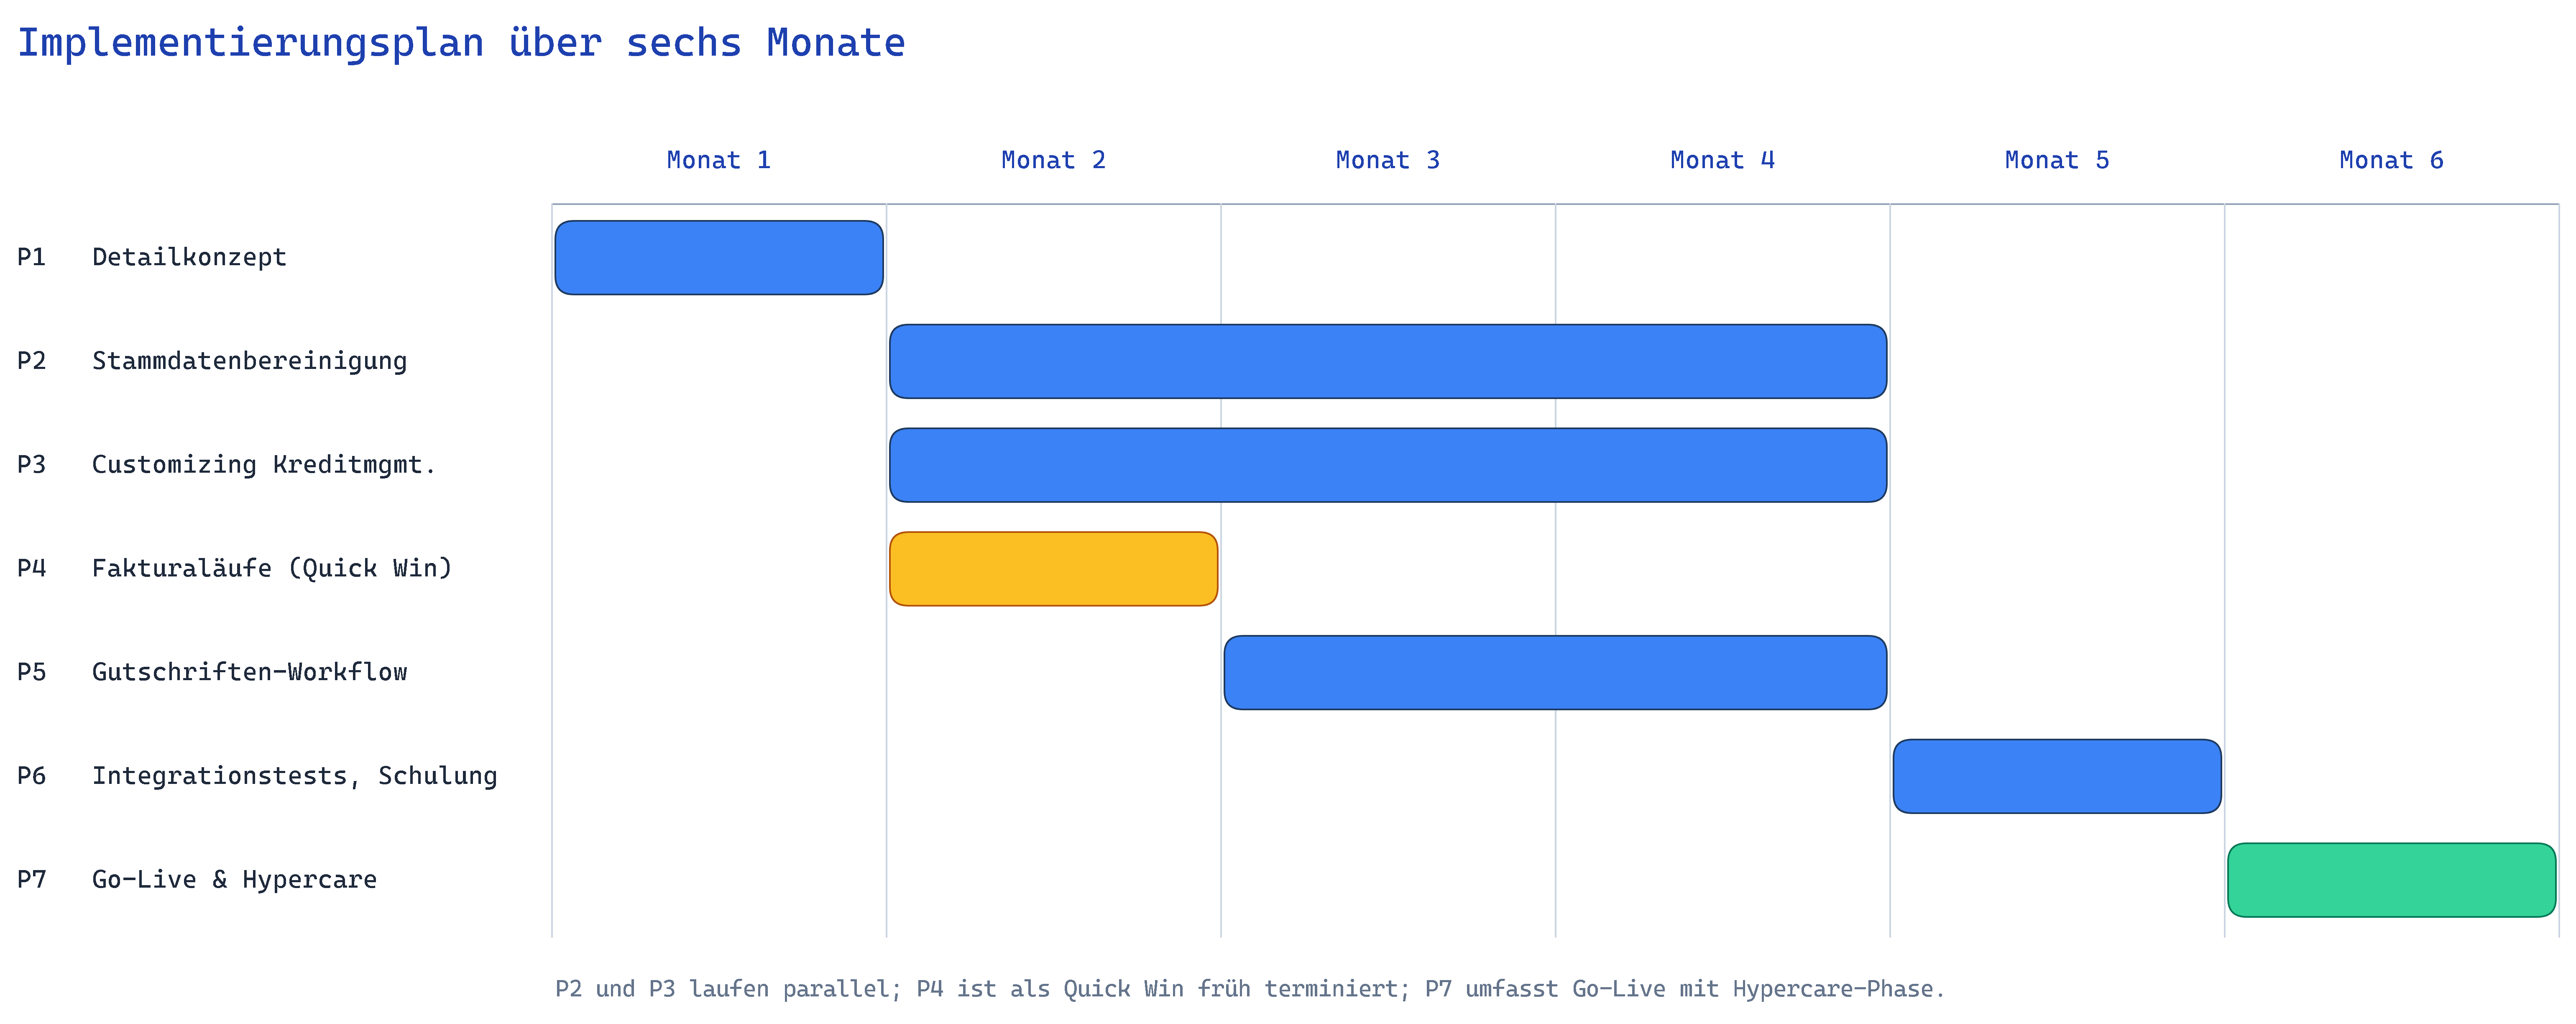
\includegraphics[width=\textwidth,height=0.36\textheight,keepaspectratio]{figures/image7.png}
\caption{Implementierungsplan über sechs Monate (Quelle: eigene Darstellung)}\label{fig:implementierungsplan}
\end{figure}

Ein iteratives, phasenweises Vorgehen ist auch aus Risikosicht geboten. Statt alle sechs Maßnahmen gleichzeitig produktiv zu setzen, werden sie nacheinander eingeführt und ihre Wirkung jeweils über das Prozessmonitoring gemessen, bevor die nächste folgt. So lässt sich etwa bei der automatisierten Kreditprüfung (M1) in einem Parallellauf beobachten, ob die neuen Regeln zu viele Aufträge blockieren oder umgekehrt Risikofälle durchlassen, und die Schwellenwerte können nachjustiert werden, bevor die manuelle Prüfung vollständig abgelöst wird. Dieses Vorgehen entspricht dem empfohlenen Phased Rollout und reduziert das Risiko, dass eine fehlerhafte Einstellung den gesamten \gls{o2c}-Prozess stört \parencite[Folie~337]{coletta2026_0206}. Inhaltlich gliedert sich das Vorhaben damit in eine Vorbereitungsphase (Detailkonzept und Priorisierung anhand der gemessenen Kennzahlen), eine Umsetzungsphase (parallele Stammdatenbereinigung und Customizing mit dem Fakturalauf als frühem Quick Win) und eine Stabilisierungsphase (Integrationstest, Schulung, Go-Live und Hypercare). Der Übergang von einer Phase zur nächsten ist jeweils an ein messbares Ergebnis geknüpft, etwa eine gesunkene Sperrquote im Parallellauf. Die Gesamtdauer von sechs Monaten ergibt sich dabei weniger aus dem technischen Aufwand der einzelnen Einstellungen, der überschaubar ist, als aus der Stammdatenbereinigung, den Testzyklen und der notwendigen Eingewöhnung der Anwender.

\section{Zeitplan und notwendige Ressourcen}\label{sec:zeitplan-ressourcen}

Für die Testphase sind Integrations-, User-Acceptance- und Regressionstests mit realistischen Testdaten vorgesehen \parencite[Folie~333 und 335]{coletta2026_0206}. Personell erfordert das Vorhaben eine interne Projektleitung (ca. 0,3 \gls{vzae}), je einen Key-User aus Vertrieb, Versand und Debitorenbuchhaltung (je ca. 0,2 \gls{vzae}), externe \gls{sd}-/\gls{fscm}-Beratung (ca. 25 Personentage) sowie die \gls{it} für Berechtigungen und Hintergrundjobs. Die externen Kosten lassen sich auf Basis marktüblicher Beratungstagessätze grob auf 60.000 bis 80.000 \euro{} schätzen. Dem stehen im modellierten Szenario rund 1.950 eingesparte Klärungsstunden pro Jahr (ca. 1,2 \gls{vzae}) sowie eine um mehrere Tage verkürzte Zeitspanne bis zur Rechnungsstellung gegenüber, die die Forderungslaufzeit unmittelbar senkt. Nach der \gls{roi}-Logik der Vorlesung amortisiert sich das Vorhaben unter diesen Annahmen bereits im ersten Jahr \parencites[Folie~343 ff.]{coletta2026_0206}[Folie~386 ff.]{coletta2026_0906}. Nach dem Go-Live werden Erfolgskriterien als Post-Go-Live-Metriken definiert und in der Hypercare-Phase proaktiv überwacht \parencite[Folie~337 und 341]{coletta2026_0206}, unmittelbar über das Prozessmonitoring aus Kapitel~\ref{sec:modifikationen-monitoring} mit den Kennzahlen aus Anhang A3.

Die Testphase verdient dabei besondere Aufmerksamkeit, weil die Maßnahmen tief in den erlöswirksamen Prozess eingreifen. Neben den funktionalen Integrationstests sind Regressionstests der angrenzenden Prozesse in Beschaffung, Bestandsführung und Debitorenbuchhaltung vorzusehen, und die neuen Kreditregeln sind an einem repräsentativen Ausschnitt historischer Aufträge zu erproben, um Fehlsperren zu vermeiden. Erst nach erfolgreichem User-Acceptance-Test durch die Key-User erfolgt der Go-Live.

Wirtschaftlich ist das Vorhaben auch unter konservativen Annahmen tragfähig. Den einmaligen externen Kosten stehen wiederkehrende Effekte gegenüber, nämlich eingesparte Klärungsstunden, eine kürzere Forderungslaufzeit und eine höhere Liefertermintreue. Weil die Liquiditätswirkung der täglichen Fakturierung sofort und ohne laufende Kosten eintritt, während die Beratungskosten nur einmalig anfallen, verschiebt sich das Kosten-Nutzen-Verhältnis bereits im ersten Jahr deutlich ins Positive. Entscheidend für die Belastbarkeit dieser Rechnung ist, dass die zugrunde liegenden Ist-Werte aus der Analyse gemessen und nicht geschätzt sind, sodass die erwarteten Einsparungen an konkreten, nachprüfbaren Kennzahlen festgemacht werden können.

\section{Risikobewertung und Managementstrategien}\label{sec:risikobewertung}

Dass \gls{erp}-nahe Projekte ihre Zeitpläne häufig überschreiten, ist empirisch gut belegt. Nur rund 21 Prozent der \gls{erp}-Implementierungen bleiben im Zeitplan. Als Hauptgründe gelten organisatorische Probleme, unrealistische Zeitpläne und Scope-Ausweitung \parencite[Panorama Consulting/Statista, zit.\ nach][Folie~211 und 213]{coletta2026_2804}. Tabelle~\ref{tab:risikomatrix} bewertet die wichtigsten Risiken und hinterlegt Gegenmaßnahmen. Hervorzuheben ist das Datenschutzrisiko, das beim Übergang von synthetischen auf reale Event-Logs entsteht. Reale Logs enthalten Benutzerkennungen und erlauben Leistungs- und Verhaltensauswertungen, Betriebsrat und Datenschutzbeauftragte sind daher früh einzubinden, und die Analysen sind auf pseudonymisierte, nicht personenbezogene Auswertungen zu beschränken.

\begin{table}[!htb]
\centering
\caption{Risikomatrix der Implementierung}\label{tab:risikomatrix}
\small
\begin{tabularx}{\textwidth}{@{}Y l l Y@{}}
\toprule
\textbf{Risiko} & \textbf{Eintritt} & \textbf{Auswirkung} & \textbf{Gegenmaßnahme} \\
\midrule
Datenqualität schlechter als angenommen (Stammdaten) & hoch & mittel & frühe Testextraktion, Bereinigung priorisieren, Puffer in P2 \\
Zu scharfe Kreditregeln blockieren Aufträge /\allowbreak{} zu laxe erhöhen Forderungsausfälle & mittel & hoch & Pilotbetrieb mit Parallellauf, Schwellenwerte iterativ justieren, Ausnahmeliste \\
Akzeptanz: Mitarbeitende fühlen sich durch Prozessdaten überwacht (reale Logs) & mittel & hoch & Pseudonymisierung, Betriebsvereinbarung, transparente Kommunikation der Ziele \\
Scope-Ausweitung (weitere Prozesse „auch noch schnell“) & mittel & mittel & Change-Request-Verfahren, Priorisierung nach Nutzwert \\
Wissensabfluss nach Beratungsende & niedrig & mittel & Dokumentation, Key-User-Schulung, Betreuungsvereinbarung \\
\bottomrule
\end{tabularx}
\end{table}

Neben diesen sachlichen Risiken ist das Veränderungsmanagement entscheidend, weil die Maßnahmen etablierte Arbeitsweisen ablösen. Die Umstellung von der manuellen auf die automatisierte Kreditfreigabe etwa entzieht der Debitorenbuchhaltung eine gewohnte Kontrollaufgabe und muss durch frühzeitige Einbindung, transparente Kommunikation der Ziele und Schulung begleitet werden. Gerade weil Process Mining das tatsächliche Verhalten sichtbar macht, ist der offene Umgang mit den Ergebnissen, verbunden mit der klaren Zusage, die Auswertung nicht zur individuellen Leistungskontrolle zu nutzen, eine Voraussetzung für die Akzeptanz im Team.


\chapter{Lessons Learned}\label{ch:lessons}


\section{Reflexion der Erfahrungen aus der Analyse}\label{sec:reflexion-erfahrungen}

Die Datenaufbereitung erwies sich als der eigentliche Engpass, selbst bei synthetischen Daten. Der Erfahrungswert, dass die Datenakquisition 60 bis 80 Prozent der Projektzeit beansprucht, bestätigte sich konkret \parencite[Folie~414]{coletta2026_3006}. In einer ersten Fassung des Simulationsmodells erzeugten nicht streng monotone Zeitstempel Schein-Kanten im entdeckten Modell. Solche Granularitäts- und Sortierprobleme treten auch bei realen \gls{sap}-Extraktionen auf, wenn tagesgenaue Felder wie \gls{augdt} mit sekundengenauen Zeitstempeln gemischt werden, und müssen vor der Discovery behoben werden, sonst analysiert man Artefakte statt Prozesse. Ebenso zeigte sich, dass die Methodenwahl kein akademisches Detail ist. Zwischen Alpha-Algorithmus und Inductive Miner lagen auf demselben Log deutliche Unterschiede (Fitness 0,646 gegenüber 0,996), und beim Soll-Abgleich machte erst der Wechsel vom Token-Replay zu Alignments die tatsächliche Konformität sichtbar (Kapitel~\ref{sec:gaps-auswirkungen}). Wer Werkzeugausgaben interpretiert, muss wissen, welcher Algorithmus mit welchen Parametern dahinterliegt. Eine zweite Grenze betrifft die Reichweite der Daten selbst. Ein Event-Log zeigt, \emph{was} geschehen ist, nicht \emph{warum}. In der Fallstudie von Adolfsson/Saleh blieb eine durchgängige manuelle Auftragsabstimmung mit dem Vertrieb unsichtbar, weil sie keine digitale Spur im \gls{erp}-System hinterließ \parencite[S.~50 und 62]{adolfsson2026o2c}. Für den synthetischen Log ist diese Grenze konstruktionsbedingt gegenstandslos, für die Übertragung auf reale Systeme jedoch zentral. Konkret zeigte sich die Bedeutung der Datenaufbereitung daran, dass erst die Erzwingung streng monoton steigender Zeitstempel je Fall die scheinbaren Rücksprünge im Modell beseitigte; ein Detail, das bei einer flüchtigen Betrachtung der Werkzeugausgabe leicht als echter Prozessschritt fehlgedeutet worden wäre. Die Lehre daraus ist, dass die Plausibilität des Event-Logs vor jeder inhaltlichen Interpretation zu prüfen ist.


\section{Erkenntnisse und Empfehlungen für ähnliche Projekte}\label{sec:erkenntnisse-empfehlungen}

Daraus folgen vier Empfehlungen: Erstens sollten Kennzahlen vor der Analyse definiert werden (Sperrquoten, Liegezeiten je Übergang, Happy-Path-Anteil, Zeit bis zur Faktura). Ohne Ziel-\gls{kpi}s erzeugt Process Mining beeindruckende, aber folgenlose Visualisierungen. Zweitens verdient die Log-Qualitätsprüfung (Monotonie, Granularität, Vollständigkeit) einen festen Platz vor jeder Discovery. Drittens gehört beim Übergang auf reale Logs der Datenschutz an den Anfang, mit Pseudonymisierung der Benutzerkennungen und früher Einbindung von Betriebsrat und Datenschutzbeauftragten (Kapitel~\ref{sec:risikobewertung}). Viertens gilt der Customizing-Leitsatz „so viel Standard wie möglich“ auch für die Behebung der Gaps. Alle sechs Maßnahmen kommen ohne Modifikation aus, was Wartbarkeit und Release-Fähigkeit erhält \parencite[Folie~248]{coletta2026_0505}. Diese Empfehlungen decken sich mit der Praxisliteratur, die rät, Analysen breit-aggregiert zu beginnen, das Werkzeug mit Interviews und Workshops zu kombinieren und den Untersuchungsumfang zunächst eng zu fassen \parencite[S.~71 f.]{adolfsson2026o2c}. Eine fünfte Erkenntnis betrifft das Zusammenspiel von Methode und Fachwissen: Process Mining liefert präzise Diagnosen, aber keine Therapien. Die Entscheidung etwa, dass die Batch-Fakturierung trotz ihrer scheinbaren Harmlosigkeit die lohnendste erste Maßnahme ist, erfordert betriebswirtschaftliches Urteilsvermögen und Kenntnis des \gls{sap}-Customizings. Das datengetriebene Vorgehen ersetzt die Prozessworkshops also nicht, es macht sie gezielter und beweisbarer \parencite[Folie~247]{coletta2026_0505}. Nicht zuletzt lohnt der Blick über den eigenen Prozess hinaus: Die Praxisliteratur und die herangezogene Fallstudie zeigen übereinstimmend, dass die größten Effekte weniger in ausgefeilteren Algorithmen als in sauberen Stammdaten und klar geschnittenen Prozessen liegen \parencites[S.~110 ff.]{nadukuru2024o2c}[S.~71 f.]{adolfsson2026o2c}. Process Mining ist damit vor allem ein Instrument, um diese unspektakulären, aber wirksamen Hebel überhaupt sichtbar und ihre Behebung messbar zu machen.


\section{Langfristige Auswirkungen auf das Unternehmen}\label{sec:langfristige-auswirkungen}

Langfristig liegt der Wert weniger in der einmaligen Diagnose als in der Verstetigung. Da Simulation und Analyse vollständig skriptbasiert und reproduzierbar sind, lässt sich dieselbe Auswertung nach jeder Prozessänderung erneut ausführen, als kontinuierliches Monitoring mit den Kennzahlen aus Anhang A3 (Kapitel~\ref{sec:modifikationen-monitoring}). Für die Organisation verschiebt das die Diskussionsgrundlage dauerhaft von Einzelmeinungen zu gemessener Evidenz. Prozessverbesserung wird überprüfbar und Prozessverantwortung messbar. Erfahrungsgemäß entsteht daraus ein kultureller Wandel: Wo Kennzahlen sichtbar sind, kehren alte Muster wie schleichend zunehmende manuelle Preisänderungen seltener unbemerkt zurück, weil jede Abweichung im Monitoring auffällt. Perspektivisch ist die Übertragung auf weitere Belegflüsse wie den Purchase-to-Pay-Prozess angelegt, für den der \gls{bpi}-Challenge-2019-Log als öffentliches Übungsfeld bereitsteht \parencite{vandongen2019bpi}.

\addtocontents{toc}{\protect\newpage}
\chapter{Zusammenfassung und Schlussfolgerungen}
\label{ch:zusammenfassung}

Die Arbeit hat untersucht, wie Prozessineffizienzen in \gls{erp}-Systemen mit Process Mining evidenzbasiert aufgedeckt werden können, anhand eines synthetischen, vollständig reproduzierbaren \gls{sap}-\gls{o2c}-Event-Logs mit bekannter Grundwahrheit. Zu F1 ist die zentrale Datenstruktur das Event-Log aus Fällen, Aktivitäten und Zeitstempeln, standardisiert im \gls{xes}-Format. In \gls{sap} \gls{s/4hana} liegt es nicht nativ vor, lässt sich aber aus den Belegtabellen (\gls{vbak}/\gls{vbap}, \gls{likp}/\gls{lips}, \gls{vbrk}/\gls{vbrp}, \gls{bkpf}/\gls{bseg}), der Belegflusstabelle \gls{vbfa} und den Änderungsbelegen \gls{cdhdr}/\gls{cdpos} rekonstruieren. Kritisch sind die Wahl der Case-ID, die Zeitstempelgranularität und die Datenqualität. Zu F2 scheiterte der Alpha-Algorithmus im empirischen Vergleich auf 12.000 Fällen an Schleifen und Rauschen (Fitness 0,646), während Heuristics Miner (0,972) und insbesondere Inductive Miner (0,996 bei Precision 0,913) brauchbare Modelle lieferten. Für den Soll-Ist-Abgleich erwiesen sich Alignments als notwendig, weil einfaches Token-Replay Abweichungsaktivitäten außerhalb des Soll-Modells übersieht. Zu F3 hat die Analyse alle sechs injizierten Störungsmuster ohne Vorwissen wiedergefunden und quantifiziert, von den Kreditsperren (34,1 \% der Fälle) bis zu den Gutschriften mit Nachlieferung (4,4 \%, Tabelle~\ref{tab:ergebnis-fitgap}). Nur 38,9 Prozent der Fälle liefen konform zum \gls{sap}-Referenzprozess.

Die abgeleiteten Maßnahmen bleiben vollständig im \gls{sap}-Standard und adressieren jede gemessene Abweichung mit einem konkreten Customizing- oder Organisationshebel. Eine Ex-post-Bewertung ihrer Effektivität entfällt studiendesignbedingt, weil die Maßnahmen abgeleitet und nicht umgesetzt wurden. An ihre Stelle tritt das Kennzahlenset in Anhang A3 mit Ist- und Zielwerten als Bewertungsmaßstab des Prozessmonitorings. Der Validierungsansatz aus bekannter Grundwahrheit und gemessener Wiederfindung belegt die Tauglichkeit der Methodenkette aus Extraktion, Discovery und Conformance Checking. Einschränkend zeigt der Log modelliertes Verhalten. Reale \gls{erp}-Daten sind unordentlicher und werfen Datenschutzfragen auf, die hier bewusst ausgeklammert wurden. Zudem hängt die Bedeutung einzelner Störungsmuster vom Geschäftskontext ab. In der Fallstudie von Adolfsson/Saleh etwa spielten Kreditsperren im Kaffeegeschäft mit stabiler Nachfrage praktisch keine Rolle \parencite[S.~51]{adolfsson2026o2c}. Die Übertragung auf ein reales System erfordert daher vor allem die in Kapitel~\ref{sec:stamm-bewegungsdaten-sap} beschriebene Extraktionsarbeit, die Algorithmen selbst sind dafür bereit.

Über die drei Forschungsfragen hinaus zeigt die Arbeit einen methodischen Mehrwert gegenüber der klassischen, workshopbasierten Fit/Gap-Analyse. Wo Letztere auf die notorisch unvollständige Dokumentation und die Erinnerung der Beteiligten angewiesen ist, stützt sich Process Mining auf die vollständige, objektive Aufzeichnung des \gls{erp}-Systems. Die Lücken werden nicht mehr geschätzt, sondern gezählt, und die Priorisierung der Maßnahmen erfolgt nach gemessener Häufigkeit und Liegezeit statt nach gefühlter Dringlichkeit. Damit wird die Fit/Gap-Analyse von einer einmaligen, subjektiven Momentaufnahme zu einem wiederholbaren, evidenzbasierten Verfahren, was gerade für das kontinuierliche Monitoring nach dem Go-Live von Bedeutung ist.

Für die Zukunft zeichnen sich drei Entwicklungen ab. Objektzentriertes Process Mining löst die Beschränkung auf eine einzige Case-ID auf und adressiert damit die in Kapitel~\ref{sec:datenstrukturen} diskutierten Konvergenz- und Divergenzprobleme \parencite[S.~3 ff.]{vanderaalst2019objectcentric}. Predictive und Prescriptive Analytics erweitern die Diagnose um Vorhersagen und Handlungsempfehlungen \parencite[Folie~470 f.]{coletta2026_1407}. Dass dieser Schritt marktreif ist, zeigt das \gls{sap}-eigene Auftragsabwicklungsmodell mit Prognosedaten (Process Forecast Data) und Side-by-Side-Simulationsberichten, mit denen sich ein simuliertes Soll-Szenario unmittelbar gegen den tatsächlichen Prozessverlauf stellen lässt \parencite[Abschnitt~3.1.16 und 3.4, S.~18 und 27--33]{sap2022samplecontent}. Auch die Fallstudie von Adolfsson/Saleh benennt die Verbindung rückblickender Analyse mit vorausschauendem Process Mining und \gls{rpa} als zentrales künftiges Feld \parencite[S.~73 f.]{adolfsson2026o2c}, und \gls{ki}-gestützte Auftragssteuerung gilt in der \gls{o2c}-Literatur zu \gls{sap} \gls{sd} als nächste Ausbaustufe \parencite[S.~111 f.]{nadukuru2024o2c}. Schließlich senken quelloffene Werkzeuge wie \gls{pm4py} die Einstiegshürde, datengetriebene Prozessanalyse ist damit nicht mehr Großkonzernen vorbehalten. Ein klar umrissener, wertschöpfungsnaher Prozess wie Order-to-Cash ist dafür der richtige erste Anwendungsfall.

Insgesamt zeigt die Arbeit einen methodischen Mehrwert gegenüber der klassischen, workshopbasierten Fit/Gap-Analyse. Deren Ergebnis hängt von der Vollständigkeit der Dokumentation und der Erinnerung der Beteiligten ab, während Process Mining sich auf die objektive Aufzeichnung des \gls{erp}-Systems stützt und die Lücken zählt statt schätzt. Für ein Unternehmen bedeutet das nicht nur eine genauere Diagnose, sondern auch eine dauerhaft wiederholbare: Dieselbe Auswertung kann nach jeder Prozessänderung erneut ausgeführt werden und macht so den Erfolg der hier abgeleiteten Maßnahmen über die Zeit messbar. Damit schließt sich der Bogen von der Datenstruktur über den Algorithmus bis zur betrieblichen Steuerung, den diese Arbeit am Beispiel des Order-to-Cash-Prozesses nachgezeichnet hat.

Für die betriebliche Praxis bedeutet dies, dass der Einstieg in Process Mining keine große Vorabinvestition erfordert. Notwendig sind ein klar abgegrenzter Prozess, ein Verständnis der zugrunde liegenden Belegtabellen und die Bereitschaft, die eigenen Abläufe an gemessenen statt an vermuteten Zahlen zu bewerten. Der \gls{o2c}-Prozess bietet dafür ideale Voraussetzungen, weil er hohe Fallzahlen, eine klare Belegstruktur und eine unmittelbare finanzielle Wirkung verbindet. Gelingt der Nachweis eines Nutzens an diesem Prozess, ist der Weg zu weiteren Anwendungsfeldern methodisch bereits geebnet.


\clearpage
\phantomsection\addcontentsline{toc}{chapter}{Anhang}
\chapter*{Anhang}


\section*{A1 Auszug aus dem Event-Log}
\addcontentsline{toc}{section}{A1 Auszug aus dem Event-Log}

Der folgende Auszug zeigt zwei repräsentative Fälle aus dem synthetischen Log: einen Happy-Path-Fall (800002) und einen Fall mit Liefersperre, Falschlieferung, Gutschrift und Nachlieferung (800347). Ein Fall mit Kreditsperre und Auftragsänderung ist in Tabelle 3 dargestellt. Alle Ressourcenkennungen sind synthetisch.

{\small
\begin{longtable}{@{}l l l l@{}}
\toprule
\textbf{Case-ID} & \textbf{Aktivität} & \textbf{Zeitstempel} & \textbf{Ressource} \\
\midrule\endhead
800002 & Auftrag angelegt & 22.09.2025 11:22:10 & VERT-11 \\
800002 & Auftrag freigegeben & 22.09.2025 11:25:10 & SYSTEM \\
800002 & Lieferung angelegt & 23.09.2025 06:30:29 & SYSTEM \\
800002 & Warenausgang gebucht & 24.09.2025 15:13:53 & LAG-03 \\
800002 & Faktura erstellt & 29.09.2025 03:10:49 & BATCH-VF06 \\
800002 & Zahlung verbucht & 03.11.2025 (tagesgenau) & FI-DEB-03 \\
800347 & Auftrag angelegt & 27.01.2026 10:44:40 & VERT-04 \\
800347 & Auftrag freigegeben & 27.01.2026 10:48:40 & SYSTEM \\
800347 & Liefersperre gesetzt & 27.01.2026 10:48:42 & SYSTEM \\
800347 & Lieferung angelegt & 03.02.2026 06:30:40 & SYSTEM \\
800347 & Warenausgang gebucht & 05.02.2026 17:54:07 & LAG-06 \\
800347 & Faktura erstellt & 09.02.2026 03:10:21 & BATCH-VF06 \\
800347 & Gutschrift erstellt & 23.02.2026 12:39:05 & VERT-04 \\
800347 & Lieferung angelegt & 24.02.2026 06:30:00 & SYSTEM \\
800347 & Warenausgang gebucht & 25.02.2026 17:09:45 & LAG-01 \\
800347 & Faktura erstellt & 02.03.2026 03:10:19 & BATCH-VF06 \\
800347 & Zahlung verbucht & 30.03.2026 (tagesgenau) & FI-DEB-01 \\
\bottomrule
\end{longtable}}


\section*{A2 Parameter des Simulationsmodells (Reproduzierbarkeit)}
\addcontentsline{toc}{section}{A2 Parameter des Simulationsmodells (Reproduzierbarkeit)}

Der Log wurde mit einem Python-Skript erzeugt (Zufallsgenerator-Seed 42, PM4Py-Version 2.7, Simulationszeitraum 01.07.2025 bis 30.06.2026, 12.000 Fälle, 84.121 Ereignisse, 11 Aktivitätstypen, Export als CSV und XES). Liegezeiten werden als Lognormalverteilungen über Arbeitstage modelliert (Wochenenden übersprungen), die Fakturierung erfolgt im wöchentlichen Sammellauf (montags 03:10 Uhr), das Zahlungsdatum ist tagesgenau modelliert (analog BSEG-AUGDT).

\begin{table}[!htb]
\centering
\small
\begin{tabularx}{\textwidth}{@{}Y l l Y@{}}
\toprule
\textbf{Muster} & \textbf{Wahrscheinlichkeit} & \textbf{Verzögerung (Median)} & \textbf{gemessen im Log} \\
\midrule
K1 Auftragsänderung (davon mehrfach) & 0,22 (0,31) & 0,6 AT je Änderung & 2.725 Fälle (22,7 \%); 814 mehrfach \\
K2 Kreditsperre + manuelle Freigabe & 0,34 & 1,8 AT & 4.086 Fälle (34,1 \%); Median 1,9 AT \\
K3 Liefersperre & 0,13 & 2,9 AT & 1.470 Fälle (12,3 \%); Median 3,9 AT bis Lieferbeleg \\
K4 Wochen-Batch-Fakturierung & alle Fälle & Sammellauf montags & Median 2,6 AT WA $\rightarrow$ Faktura \\
K5 Fakturasperre (manuelle Preise) & 0,077 & 1,5 AT & 944 Fälle (7,9 \%) \\
K6 Gutschrift /\allowbreak{} Nachlieferung & 0,045 /\allowbreak{} 0,04 & 6,0 /\allowbreak{} 1,5 AT & 532 /\allowbreak{} 471 Fälle \\
Zahlungsziel-Verhalten & -- & 38 Tage (lognormal) & Median 38 Tage Faktura $\rightarrow$ Zahlung \\
\bottomrule
\end{tabularx}
\end{table}


\section*{A3 Kennzahlen des Prozessmonitorings}
\addcontentsline{toc}{section}{A3 Kennzahlen des Prozessmonitorings}

\begin{table}[!htb]
\centering
\small
\begin{tabularx}{\textwidth}{@{}Y l l Y@{}}
\toprule
\textbf{Kennzahl} & \textbf{Ist (gemessen)} & \textbf{Zielwert nach Maßnahmen} & \textbf{Wesentlicher Hebel} \\
\midrule
Anteil Fälle mit Kreditsperre & 34,1 \% & ca. 10 \% & M1 automatisierte Kreditprüfung \\
Anteil Fälle mit Liefersperre & 12,3 \% & ca. 5 \% & M2 Stammdatenqualität \\
Liegezeit Warenausgang $\rightarrow$ Faktura (Median) & 2,6 AT & ca. 0,5 AT & M3 tägliche Fakturierung \\
Fälle mit Fakturasperre & 944 (7,9 \%) & \textless{} 350 & M4 Konditionspflege, Berechtigungen \\
Manueller Klärungsaufwand p. a. (geschätzt) & ca. 1.950 h & \textless{} 700 h & M1--M5 \\
Durchlaufzeit Auftrag $\rightarrow$ Faktura (Median) & 5,8 AT & ca. 4,5 AT & M1--M4 \\
Happy-Path-Anteil (konforme Fälle) & 38,9 \% & \textgreater{} 65 \% & alle Maßnahmen \\
Anzahl Prozessvarianten & 85 & \textless{} 40 & alle Maßnahmen \\
\bottomrule
\end{tabularx}
\end{table}



\clearpage
\phantomsection\addcontentsline{toc}{section}{Literaturverzeichnis}
\section*{Literaturverzeichnis}

\begingroup\setlength{\parindent}{0pt}\setlength{\parskip}{0.5em}

\noindent\hangindent=1.5em Adolfsson, J./Saleh, D. (2026): Analyzing Order-to-Cash Using Process Mining. A Case Study in Collaboration with Paulig, Master's Thesis, Department of Technology Management and Economics, Chalmers University of Technology, Gothenburg.\par

\noindent\hangindent=1.5em Berti, A./van Zelst, S. J./van der Aalst, W. M. P. (2019): Process Mining for Python (PM4Py). Bridging the Gap Between Process- and Data Science, in: ICPM Demo Track 2019, CEUR Workshop Proceedings, Bd. 2374.\par

\noindent\hangindent=1.5em Coletta, S. (2026a): ERP-Systeme. Vorlesungsunterlagen vom 03.03.2026, FOM Hochschule für Oekonomie \& Management, Essen, Sommersemester 2026.\par

\noindent\hangindent=1.5em Coletta, S. (2026b): ERP-Systeme. Vorlesungsunterlagen vom 10.03.2026, FOM Hochschule für Oekonomie \& Management, Essen, Sommersemester 2026.\par

\noindent\hangindent=1.5em Coletta, S. (2026c): ERP-Systeme. Vorlesungsunterlagen vom 28.04.2026, FOM Hochschule für Oekonomie \& Management, Essen, Sommersemester 2026.\par

\noindent\hangindent=1.5em Coletta, S. (2026d): ERP-Systeme. Vorlesungsunterlagen vom 05.05.2026, FOM Hochschule für Oekonomie \& Management, Essen, Sommersemester 2026.\par

\noindent\hangindent=1.5em Coletta, S. (2026e): ERP-Systeme. Vorlesungsunterlagen vom 19.05.2026, FOM Hochschule für Oekonomie \& Management, Essen, Sommersemester 2026.\par

\noindent\hangindent=1.5em Coletta, S. (2026f): ERP-Systeme. Vorlesungsunterlagen vom 02.06.2026, FOM Hochschule für Oekonomie \& Management, Essen, Sommersemester 2026.\par

\noindent\hangindent=1.5em Coletta, S. (2026g): ERP-Systeme. Vorlesungsunterlagen vom 09.06.2026, FOM Hochschule für Oekonomie \& Management, Essen, Sommersemester 2026.\par

\noindent\hangindent=1.5em Coletta, S. (2026h): ERP-Systeme. Vorlesungsunterlagen vom 23.06.2026, FOM Hochschule für Oekonomie \& Management, Essen, Sommersemester 2026.\par

\noindent\hangindent=1.5em Coletta, S. (2026i): ERP-Systeme. Vorlesungsunterlagen vom 30.06.2026, FOM Hochschule für Oekonomie \& Management, Essen, Sommersemester 2026.\par

\noindent\hangindent=1.5em Coletta, S. (2026j): ERP-Systeme. Vorlesungsunterlagen vom 14.07.2026, FOM Hochschule für Oekonomie \& Management, Essen, Sommersemester 2026.\par

\noindent\hangindent=1.5em Gronau, N. (2014): Enterprise Resource Planning. Architektur, Funktionen und Management von ERP-Systemen, 3. Aufl., De Gruyter Oldenbourg, Berlin/München.\par

\noindent\hangindent=1.5em IEEE (2016): IEEE Standard for eXtensible Event Stream (XES) for Achieving Interoperability in Event Logs and Event Streams, IEEE Std 1849-2016, IEEE, New York.\par

\noindent\hangindent=1.5em Leemans, S. J. J./Fahland, D./van der Aalst, W. M. P. (2013): Discovering Block-Structured Process Models from Event Logs. A Constructive Approach, in: Colom, J.-M./Desel, J. (Hrsg.): Application and Theory of Petri Nets and Concurrency, LNCS 7927, Springer, Berlin/Heidelberg, S. 311--329.\par

\noindent\hangindent=1.5em Nadukuru, S./Dandu, M. M. K./Balasubramaniam, V. S./Renuka, A./Goel, O. (2024): Enhancing Order to Cash Processes in SAP Sales and Distribution, in: Darpan International Research Analysis, 12. Jg., Nr. 1, S. 108--139.\par

\noindent\hangindent=1.5em Peters, R./Nauroth, M. (2019): Process-Mining. Geschäftsprozesse: smart, schnell und einfach, Springer Gabler, Wiesbaden.\par

\noindent\hangindent=1.5em Reinkemeyer, L. (Hrsg.) (2020): Process Mining in Action. Principles, Use Cases and Outlook, Springer, Cham.\par

\noindent\hangindent=1.5em Rozinat, A./van der Aalst, W. M. P. (2008): Conformance Checking of Processes Based on Monitoring Real Behavior, in: Information Systems, 33. Jg., Nr. 1, S. 64--95.\par

\noindent\hangindent=1.5em SAP AG (2013): Sales -- A/R. Sales Order to Cash, Schulungsunterlage TB1000 (SAP Business One, Version 9.0), SAP AG, Walldorf.\par

\noindent\hangindent=1.5em SAP SE (2022): Sample Content for Process Mining on SAP S/4HANA -- Order to Cash. Processes and Functions supporting Sample Business Scenarios, SAP Profitability and Performance Management, Dokumentversion 3.0 SP20 (2022-12-20), SAP SE, Walldorf.\par

\noindent\hangindent=1.5em Scheibler, J. (2021): Vertrieb mit SAP S/4HANA. Das Praxishandbuch, Rheinwerk, Bonn.\par

\noindent\hangindent=1.5em van der Aalst, W. M. P. (2016): Process Mining. Data Science in Action, 2. Aufl., Springer, Berlin/Heidelberg.\par

\noindent\hangindent=1.5em van der Aalst, W. M. P. (2019): Object-Centric Process Mining. Dealing with Divergence and Convergence in Event Data, in: Ölveczky, P. C./Salaün, G. (Hrsg.): Software Engineering and Formal Methods (SEFM 2019), LNCS 11724, Springer, Cham, S. 3--25.\par

\noindent\hangindent=1.5em van der Aalst, W. M. P. et al. (2012): Process Mining Manifesto, in: Daniel, F./Barkaoui, K./Dustdar, S. (Hrsg.): Business Process Management Workshops (BPM 2011), LNBIP 99, Springer, Berlin/Heidelberg, S. 169--194.\par

\noindent\hangindent=1.5em van der Aalst, W. M. P./Weijters, A. J. M. M./Măruşter, L. (2004): Workflow Mining. Discovering Process Models from Event Logs, in: IEEE Transactions on Knowledge and Data Engineering, 16. Jg., Nr. 9, S. 1128--1142.\par

\noindent\hangindent=1.5em van Dongen, B. F. (2019): BPI Challenge 2019. Event Log, 4TU.ResearchData, Eindhoven.\par

\noindent\hangindent=1.5em Weijters, A. J. M. M./van der Aalst, W. M. P. (2003): Rediscovering Workflow Models from Event-Based Data Using Little Thumb, in: Integrated Computer-Aided Engineering, 10. Jg., Nr. 2, S. 151--162.\par



\endgroup


\end{document}
